%% =========================================================================
%%  Core Signatures and Inversions --- Wilmott magazine version, revision 1
%%
%%  Revised after the Wilmott review of August 2026 (MS WP-1259). The paper
%%  is self-contained: Proposition 1 is proved in Appendix B, the
%%  substitution rules through level 5 are in Appendix A, the two-piece
%%  closed forms in Appendix C, and the term-structure application is
%%  Section 5; the Python code is in the public GitHub repository, not
%%  printed. No pointer to any notebook, preprint or work in preparation.
%% =========================================================================

\documentclass[11pt,english]{article}
\usepackage[T1]{fontenc}
\usepackage[utf8]{inputenc}
\usepackage[table]{xcolor}
\usepackage{colortbl}
\usepackage{babel}
\usepackage{cprotect}
\usepackage{float}
\usepackage{url}
\usepackage{amsmath}
\usepackage{amssymb}
\usepackage{amsthm}
\usepackage{graphicx}
\usepackage{booktabs}
\usepackage[a4paper]{geometry}
\geometry{verbose,tmargin=2.5cm,bmargin=2.5cm,lmargin=2.5cm,rmargin=2.5cm,footskip=1cm}
\usepackage{fancyhdr}
\pagestyle{fancy}
\usepackage[pdfusetitle,
 bookmarks=true,bookmarksnumbered=false,bookmarksopen=false,
 breaklinks=false,pdfborder={0 0 1},backref=false,colorlinks=false]
 {hyperref}
\hypersetup{colorlinks=true,citecolor=blue}

\makeatletter
\providecommand{\tabularnewline}{\\}
\makeatother

\usepackage{lastpage}
\usepackage{breakcites}
\lhead{}\chead{}\rhead{}
\lfoot{}\cfoot{\thepage\ / \pageref{LastPage}}\rfoot{}
\renewcommand{\headrulewidth}{0pt}
\usepackage{indentfirst}

\makeatletter
\providecommand*{\shuffle}{\mathbin{\mathpalette\shuffle@{}}}
\newcommand*{\shuffle@}[2]{%
  \sbox0{$#1\vcenter{}$}%
  \kern .15\ht0
  \rlap{\vrule height .25\ht0 depth 0pt width 2.5\ht0}%
  \raise.1\ht0\hbox to 2.5\ht0{%
    \vrule height 1.75\ht0 depth -.1\ht0 width .17\ht0
    \hfill
    \vrule height 1.75\ht0 depth -.1\ht0 width .17\ht0
    \hfill
    \vrule height 1.75\ht0 depth -.1\ht0 width .17\ht0}%
  \kern .15\ht0
}
\makeatother

\usepackage{xurl}
\newcommand{\nbfile}[1]{\nolinkurl{#1}}

%% Allow TeX to expand justification in difficult paragraphs rather
%% than letting them bleed into the right margin.
\setlength{\emergencystretch}{3em}

\newtheorem{theorem}{Theorem}
\newtheorem{proposition}[theorem]{Proposition}
\newtheorem{corollary}[theorem]{Corollary}
\newtheorem{lemma}[theorem]{Lemma}
\theoremstyle{definition}
\newtheorem{example}[theorem]{Example}
\theoremstyle{remark}
\newtheorem{remark}[theorem]{Remark}

%% CUT VARIANT (2026-09-20): Appendices A, B and C and the proofs of the three stability
%% theorems moved to the supplement; Example obstruction and Lemma concat dropped, Corollary
%% regression-bound kept with a shorter discussion; see make_cut_version.py. Supplement:
%% supplement CoreSignaturesAndInversions_Wilmott_R1_Supplement_2026-09.tex.
\begin{document}

\title{Core Signatures and Inversions}
\author{Marcos Costa Santos Carreira\thanks{marcoscscarreira@gmail.com}}
\date{First version May 29, 2026; revised September 20, 2026}
\maketitle


\begin{abstract}
Core signatures retain the entries of a truncated path signature
indexed by Lyndon words. Classical shuffle-algebra results show that
these entries are polynomial coordinates: they carry the same
information as the truncated signature, with the dimension of the
log signature and without a Lie-basis projection. We give an explicit
elimination procedure and substitution rules through level five, and
study recovery of time-augmented paths from these coordinates.
For two linear segments we characterise exact recovery by a
compatibility condition and an admissible breakpoint. The coordinates
containing one value increment are moments of that increment; this
gives exact polynomial recovery and a finite-level stability estimate
on bounded polynomial families. A rank condition gives local recovery
on smooth parameterised families. We also calculate the covariance of
the moment coordinates under additive Brownian-bridge noise.
Two counterexamples delimit the theory: undamped factorial weighting
can make the all-level residual infinite, and signature depth cannot
remove the approximation barrier of a fixed piecewise-linear class.
A damped all-level metric recovers the uniform topology on an anchored
class with a common Lipschitz bound, without asserting Sobolev norm
equivalence. A Python implementation and two interest-rate curves illustrate
the distinction between exact recovery, stable identification and
approximation by signature regression.

\medskip{}
\textit{Keywords}: signatures; log signatures; Lyndon words; signature
inversion; term-structure modelling
\end{abstract}

%% =========================================================================
\section{Introduction}
%% =========================================================================

Term structures --- interest rates, implied volatilities, futures curves
--- are functions of time-to-maturity that practitioners want to compress
into a small number of geometric features. Principal components provide linear summaries of a collection of curves.
Signatures instead encode an individual curve through iterated integrals
and respect concatenation. For a path $X:[a,b]\to\mathbb{R}^{d}$,
the signature $S(X)_{a,b}$ collects all iterated integrals along
$X$ into a single tensor series; the full series determines $X$, with its starting point fixed, up to
tree-like equivalence (Section \ref{sec:Inversion}), and truncated at
level $m$ it provides a finite-dimensional encoding of $X$. The
truncated signature contains redundancies coming
from the shuffle relations, and the standard remedy is the log signature
--- whose dimension is that of the free nilpotent Lie algebra $\mathfrak{g}^{m}(\mathbb{R}^{d})$,
typically computed in practice through Reizenstein's \texttt{iisignature}
library \cite{iisignature,iisignature 1004,log signatures}.


The question studied here is when a reduced set of signature entries
permits identification and stable recovery of a time-augmented path.
We first make the coordinate construction explicit: a lexicographic
shuffle elimination retains exactly the Lyndon entries, and the
remaining entries are polynomial functions of them. Next we separate
three inverse problems. Exact recovery asks whether a target belongs
to the signature image of a specified path class; we give a complete
level-three criterion for two time-ordered segments. Identification
asks whether different members of that class have different
coordinates; polynomial moments and a local rank condition provide
two answers. Stability asks how changes in coordinates control changes
in the recovered path; on a bounded polynomial family we prove a
two-sided estimate with fixed positive weights.

For longer piecewise-linear paths we use weighted nonlinear
least squares. This computation motivates, but is not covered by,
every stability result above. We distinguish the target-magnitude
normalisation used in the experiments from covariance weighting
justified by a Brownian-bridge observation model. We then give
obstructions to unrestricted all-level weighting and to excessive
approximation-rate claims, and prove a topological stability result
for a damped all-level metric. The Brazilian DI futures curve and
the US Treasury curve illustrate how truncation, representation and
the approximation class affect the numerical reconstruction.

The paper is organised as follows. Section \ref{sec:Signatures} recalls
signatures, the shuffle product and Chen's identity. Section
\ref{sec:Core} defines core signatures and states their identification
with Lyndon coordinates, proved in Section S3 of the supplement. Section
\ref{sec:Inversion} inverts core signatures into piecewise-linear
paths, from the two-segment closed forms to the regression, and
develops the moment identity, finite-level stability, covariance weighting
and an all-level metric with a continuity guarantee. Section \ref{sec:Curves}
illustrates the inversion on the two curves. The supplementary
material submitted with this paper holds the tabulated substitution
rules (Section S1), the closed-form two-segment solutions and the
three-segment matching system (S2), the proof of Proposition
\ref{prop:core-is-lyndon} (S3) and the full proofs of the three
stability theorems (S4); the text names the section where each is
supplied.

The structural identification of core entries with Lyndon coordinates
follows from results that are classical in the algebraic-combinatorics
literature (\cite{Reutenauer}, the Lyndon basis theorem and Radford's
theorem) and in the rough-paths literature (\cite{varieties}, the
universal variety $G^{n}(\mathbb{R}^{d})$). The coordinate theorem is
theirs; our contribution is the computational packaging: naming the
subset, exhibiting an explicit shuffle-product elimination that
produces it, tabulating the substitution rules $Q_{m}$, and using these
coordinates for Chen-based inversion. For previous signature-inversion
algorithms see \cite{inversion}.

After our 2023 preprint, \cite{macaulay2} introduced a Macaulay2 package
(\texttt{PathSignatures}) whose \texttt{lyndonShuffle} method implements
the same Lyndon-shuffle decomposition that underlies our substitution
rules $Q_{m}$. In their Section 6 they use the term \emph{core signature
tensor} with a different meaning: the signature of a base path that
generates a family by linear transformation, suited to the algebraic
geometry of signature varieties rather than to Chen-based inversion
of individual signatures. The terminology overlap is unfortunate but
the constructions are distinct. A parallel Julia/OSCAR implementation
is in \cite{signaturetensorsjl}.

%% =========================================================================
\section{Signatures\label{sec:Signatures}}
%% =========================================================================

A path is a continuous map $X:[a,b]\to\mathbb{R}^{d}$ of bounded variation;
we reparametrise to $[0,1]$ when convenient. The signature truncated
at level $m$ is
\begin{equation}
S^{(\leq m)}(X)_{a,b}\;=\;\Bigl(\,1,\;S^{i_{1}},\;S^{i_{1},i_{2}},\;\ldots,\;S^{i_{1},\ldots,i_{m}}\,\Bigr)\,,\qquad i_{k}\in\{1,\ldots,d\}\,,
\end{equation}
with level-$k$ entries
\begin{equation}
S^{i_{1},\ldots,i_{k}}\;=\;\int_{a}^{b}\int_{a}^{t_{k}}\cdots\int_{a}^{t_{2}}dX_{t_{1}}^{i_{1}}\,\cdots\,dX_{t_{k}}^{i_{k}}\,.\label{eq:IteratedIntegral}
\end{equation}
For a single line segment with slopes $(\beta_{1},\ldots,\beta_{d})$
over an interval of length $T$, every entry has a closed form:
\begin{equation}
S^{i_{1},\ldots,i_{k}}\;=\;\frac{\beta_{i_{1}}\cdots\beta_{i_{k}}T^{k}}{k!}\,.\label{eq:LineSignature}
\end{equation}
This is the building block we will use throughout the inversion.

\paragraph{Shuffle product.}
A $(p,q)$-shuffle of two ordered sequences of lengths $p,q$ is an
interleaving that preserves the relative order within each sequence;
$I\shuffle J$ denotes the multiset of all shuffles of multi-indices
$I$ and $J$. The fundamental shuffle identity --- valid for any
path --- is
\begin{equation}
S^{I}\cdot S^{J}\;=\;\sum_{K\in\,I\shuffle J}S^{K}\,.\label{eq:ShuffleProduct}
\end{equation}
Equation \eqref{eq:ShuffleProduct} is the algebraic engine of Section
\ref{sec:Core}: it provides the relations that reduce the truncated
signature to its core.

\paragraph{Chen's identity.}
For consecutive paths $X:[a,b]\to\mathbb{R}^{d}$ and $Y:[b,c]\to\mathbb{R}^{d}$,
the concatenation $Z=X*Y$ has signature
\begin{equation}
S(Z)_{a,c}\;=\;S(X)_{a,b}\otimes S(Y)_{b,c}\,,\quad\text{or componentwise}\quad z_{i_{1},\ldots,i_{k}}\;=\;\sum_{j=0}^{k}x_{i_{1},\ldots,i_{j}}\cdot y_{i_{j+1},\ldots,i_{k}}\,,\label{eq:ChenIndex}
\end{equation}
with the conventions $x_{\emptyset}=y_{\emptyset}=1$. The componentwise
form allows us to compute individual entries of $Z$ without rebuilding
the full concatenated signature --- the basis of the inversion algorithm
in Section \ref{sec:Inversion}.

%% =========================================================================
\section{Core Signatures\label{sec:Core}}
%% =========================================================================

The shuffle relations mean that not every entry of the truncated signature
carries new information. A standard parsimonious encoding represents
the log signature in a basis of the free Lie algebra, such as a Hall
basis. The core construction instead selects a subset of
the truncated signature itself --- the \emph{core elements} --- has
the same dimension and the same information content as the log signature,
can be read directly from $S(X)$, and admits an explicit structural
characterisation in terms of Lyndon words.

\subsection{Core variables via the shuffle product}

Let $V_{m}=\{s_{w}:|w|=m\}$ denote the set of signature entries at
level $m$, and let $C_{m}$ be the \emph{core set up to level} $m$,
defined by processing words at each level in increasing lexicographic
order and retaining an entry when the shuffle identities do not express
it as a polynomial in earlier entries at that level and entries at lower
levels. Section S3 of the supplement proves that this procedure retains the Lyndon words.
For $d=2$, the recursive application of \eqref{eq:ShuffleProduct}
at level 3 gives the following elimination relations
\[
\begin{array}{l}
3s_{1,1,1}-s_{1}s_{1,1}\,,\quad-s_{2}s_{1,1}+s_{1}s_{2,1}+s_{1,1,2}-s_{2,1,1}\,,\\
-s_{1}s_{2,1}+s_{1,2,1}+2s_{2,1,1}\,,\quad-s_{2}s_{1,2}+s_{2}s_{2,1}+2s_{1,2,2}-2s_{2,2,1}\,,\\
-s_{2}s_{2,1}+s_{2,1,2}+2s_{2,2,1}\,,\quad3s_{2,2,2}-s_{2}s_{2,2}\,.
\end{array}
\]
After eliminating six variables in terms of $C_{2}=\{s_{1},s_{2},s_{1,2}\}$
and processing the level-three words in lexicographic order, two entries
remain free:
\[
C_{3}\;=\;C_{2}\,\cup\,\{s_{1,1,2},\,s_{1,2,2}\}\,.
\]
Repeating the construction at higher levels yields the core sizes
for $d=2$:
\begin{equation}
|C_{m}|\,\text{ for }m=1,\ldots,6\;=\;2,\,3,\,5,\,8,\,14,\,23\,,\label{eq:CoreSizesD2}
\end{equation}
matching the log-signature column of Reizenstein's tables. For $d=3$
the corresponding counts are $3,6,14,32,80,196$. The
Lyndon multi-indices that constitute $C_{4}$ and $C_{5}$ are listed
in Section S1 of the supplement (and those of $C_{6}$ in Table
\ref{tab:Lyndon-d2}), where the 48 substitution rules $Q_{m}$ for
$m\leq5$ are tabulated in full. The same elimination procedure extends
to higher levels and larger alphabets; the tables stop at level five
for $d=2$.


The companion module \texttt{coresig.py} in the repository (see the
code-and-data statement) implements the binary word index and the
piecewise-linear signature: \texttt{Words} identifies Lyndon words,
\texttt{segment\_signature} evaluates a single segment,
\texttt{chen} concatenates signatures, and
\texttt{piecewise\_signature} computes the full truncated signature of
a piecewise-linear path and selects the core. The module uses NumPy
and SciPy \cite{numpy,scipy}. The script
\texttt{listing2\_rules\_check.py} checks two rules of Section S1 of
the supplement on a random four-segment path.

\begin{table}[H]
\centering
\begin{tabular}{|r|r|r|r|r|r|r|}
\hline
$m$ & $d=2$ sig & $d=2$ core/log & $d=3$ sig & $d=3$ core/log & $d=4$ sig & $d=4$ core/log\tabularnewline
\hline\hline
1 & 2 & 2 & 3 & 3 & 4 & 4\tabularnewline\hline
2 & 6 & 3 & 12 & 6 & 20 & 10\tabularnewline\hline
3 & 14 & 5 & 39 & 14 & 84 & 30\tabularnewline\hline
4 & 30 & 8 & 120 & 32 & 340 & 90\tabularnewline\hline
5 & 62 & 14 & 363 & 80 & 1364 & 294\tabularnewline\hline
6 & 126 & 23 & 1092 & 196 & 5460 & 964\tabularnewline\hline
\end{tabular}
\caption{Sizes of signatures and core signatures at low levels. Core sizes
coincide with the log-signature sizes of \cite{log signatures}.\label{tab:Sizes}}
\end{table}

\subsection{Core elements as Lyndon coordinates}

The numerical coincidence $|C_{m}|=\dim\mathfrak{g}^{m}(\mathbb{R}^{d})$
and the entries retained by lexicographic elimination
are consequences of the Lyndon basis of the free Lie algebra. Fix
the lexicographic order on $\mathcal{A}=\{1,\ldots,d\}$; a non-empty
word $w$ is a \emph{Lyndon word} if $w<vu$ for every non-trivial
factorisation $w=uv$. For $d=2$, the Lyndon words of length $\leq6$
on $\{1,2\}$ are listed in Table \ref{tab:Lyndon-d2}; comparison
with $C_{6}$ shows the multi-indices agree exactly.

\begin{table}[H]
\centering
\begin{tabular}{|c|l|}
\hline
Length & Lyndon words on $\{1,2\}$\tabularnewline
\hline\hline
1 & $1$, $2$\tabularnewline\hline
2 & $12$\tabularnewline\hline
3 & $112$, $122$\tabularnewline\hline
4 & $1112$, $1122$, $1222$\tabularnewline\hline
5 & $11112$, $11122$, $11212$, $11222$, $12122$, $12222$\tabularnewline\hline
6 & $111112$, $111122$, $111212$, $111222$, $112122$, $112212$, $112222$, $121222$, $122222$\tabularnewline\hline
\end{tabular}
\caption{Lyndon words on $\{1,2\}$ up to length 6. These are exactly the multi-indices
of the core variables.\label{tab:Lyndon-d2}}
\end{table}

\begin{proposition}[Core variables are Lyndon coordinates]
\label{prop:core-is-lyndon} The core sets $C_{m}$ identified by
the shuffle-product computation are exactly the Lyndon words on $\{1,\ldots,d\}$
of length $\leq m$. The corresponding $\sigma_{w}$ form a transcendence
basis for the coordinate ring of the universal variety $G^{m}(\mathbb{R}^{d})$,
and the substitution rules $Q_{m}$ are the explicit form of the corresponding
Radford isomorphism truncated at level $m$.
\end{proposition}

The proof uses three classical ingredients: the Lyndon basis theorem
for the free Lie algebra (\cite{Reutenauer} Theorem 5.1), Poincaré--Birkhoff--Witt,
and Radford's theorem that the shuffle algebra is the free commutative
algebra on Lyndon words (\cite{Reutenauer} Theorem 6.1). Together
they identify the Lyndon-indexed signature entries with algebraically
independent coordinates on the universal variety $G^{n}(\mathbb{R}^{d})$
studied in \cite{varieties}. The triangular identity associated with
Lyndon factorisation explains why lexicographic elimination retains
these entries. The proof is given in Section S3 of the supplement.

\subsection{Witt formula and the Pascal-triangle structure}

The number of Lyndon words of length $n$ on a $d$-letter alphabet
is given by Witt's formula (\cite{Reutenauer} Section 4):
\begin{equation}
\ell_{d}(n)\;=\;\frac{1}{n}\sum_{k\,\mid\,n}\mu\!\left(\tfrac{n}{k}\right)\,d^{\,k}\,,\label{eq:Witt}
\end{equation}
where $\mu$ is the Möbius function. For $d=2$ this gives the sequence
$2,1,2,3,6,9,18,30,\ldots$ whose cumulative sums match \eqref{eq:CoreSizesD2}.
The multi-graded refinement of \eqref{eq:Witt} --- counting Lyndon
words on $\{1,2\}$ with prescribed numbers of $1$s and $2$s --- recovers
the Pascal-triangle distribution we observed empirically in the substitution
rules.

%% =========================================================================
\section{Inversion of Core Signatures\label{sec:Inversion}}
%% =========================================================================


We use Chen's identity \eqref{eq:ChenIndex} to seek a piecewise-linear
path with prescribed core coordinates. Exact recovery requires all
matching equations to hold and the parameters to define an admissible
path. Solving a square subsystem alone need not satisfy the omitted
equations. When exact recovery is unavailable, we minimise a weighted
residual over a chosen path class. We develop the time-ordered case
$X(t)=(t,f(t))$, with $f(0)$ fixed, and also give planar examples.

\paragraph{Related work on the inversion problem.}
Three recent papers from the Berlin/TU group develop the inversion
problem from an algebraic-geometric angle that complements ours. \cite{splines}
generalise the piecewise-linear and polynomial classes of \cite{varieties}
to piecewise polynomial paths and splines, and introduce the \emph{path
recovery degree} (Definition 6.1) as the number of complex points
in a generic fibre of the signature map, that is, the number of paths
in a class sharing one full truncated signature. For $d=2$ at level
$k=4$, their Table 3 records the
recovery degree as $4$ for piecewise linear paths with four segments
and $48$ for the degree-four polynomial class. \cite{tensorlearning}
gives an $O(d^{4})$ algorithm for the level-3 $d$-segment piecewise
linear case using Gauss transformations on signature tensors as a
tensor analogue of congruence normal forms, outperforming Gröbner-basis
methods. \cite{barycenters} treats the adjacent problem of path recovery
from \emph{barycenters} of multiple signatures, relevant when the
input is an expected signature.


The time-ordered setting gives explicit recovery formulas for two
segments and a polynomial matching system for three (Section S2 of
the supplement). It also exposes a moment map inside the
signature. This map yields the identification and stability results
below and explains which part of signature regression is moment
matching. A comparison with a path-space fitting objective is a
separate question: neither the moment identity nor identifiability
implies equality of the two minimisers.

\begin{remark}[What the signature determines]
\label{rem:treelike}
A theorem of \cite{HamblyLyons} identifies the ambiguity of the full
signature: for paths of bounded variation with a fixed starting point,
equality of signatures is equivalent to \emph{tree-like equivalence}.
Immediate out-and-back excursions are a simple example of this
equivalence. Each
equivalence class contains a tree-reduced path, unique up to
reparametrisation, which is the representative of minimal length. Two consequences organise this
section. First, a time-ordered path $X(t)=(t,f(t))$ cannot retrace
itself, since its first coordinate is strictly increasing, so it is
tree-reduced and its full signature determines $f$ once $f(0)$ is
fixed (the signature sees only $df$). Truncating the signature turns
this into an inverse problem with its own questions --- whether a
finite-segment path with the truncated target exists, how many there
are (the recovery degrees of \cite{splines}), and how stably they
depend on the target --- which the rest of this section takes up
one at a time. Second, the coordinate $t$ in $X(t)=(t,f(t))$ supplies
a specified clock, and the entries with a single letter 2 are moments
of the increment in that clock (Proposition
\ref{prop:moment-identity}). For a general planar path $(x(s),y(s))$
neither coordinate need be monotone, and the moment interpretation is
unavailable. Its signature is invariant under increasing
reparametrisation \cite{Primer} and retains the order of traversal.
Section \ref{subsec:Regression} recovers polygonal approximations to
the semicircle and the digit 5 directly from their planar core
entries. A clock can also be retained as an additional coordinate,
giving $(s,x(s),y(s))$ on the three-letter alphabet; its mixed entries
then record the chosen timing. The following proposition records the
invariance under an inserted out-and-back excursion.
\end{remark}

\begin{proposition}[Retracings are invisible]
\label{prop:retracing}
Let $P$ be a polygonal path in $\mathbb{R}^{d}$ and let $P'$ be obtained
from $P$ by inserting at any knot an excursion along a segment $v$ and
straight back, $v$ then $-v$. Then $S(P')=S(P)$ at every level. In
particular, for $n\geq3$ the map from $n$-segment polygons with fixed
endpoints to their signatures is not injective, and for every level $m$
the regression objective \eqref{eq:weighted-regression}, as a function
of the $n$-segment polygon, is constant along every $d$-parameter
family $\{P\text{ with }v,-v\text{ inserted}:v\in\mathbb{R}^{d}\}$; it
has flat directions of dimension $d$ at every polygon that contains a
retracing. No such family exists for time-ordered paths, whose segments
all have positive time increment.
\end{proposition}

\begin{proof}
The signature of a straight segment with increment $v$ is
$\exp(v)=\sum_{k\geq0}v^{\otimes k}/k!$ (this is \eqref{eq:LineSignature}),
and $\exp(v)\otimes\exp(-v)=1$ in the tensor algebra. By Chen's identity
\eqref{eq:ChenIndex} the excursion contributes the factor
$\exp(v)\otimes\exp(-v)=1$ to the product of segment signatures, so
$S(P')=S(P)$. A time-ordered path has $v_{1}>0$ on every segment, so no
segment can be followed by its reverse.
\end{proof}


The self-crossing fits of Figure \ref{fig:digit5_5} are not exact
retracings; Proposition \ref{prop:retracing} exhibits the ambiguity
that motivates the regularisation. Along an exact inserted out-and-back
family the signature is constant, while the added length is $2|v|$;
a positive penalty on excess length therefore favours $v=0$ on that
family. In a general penalised fit, however, length and signature
error are traded off.

\subsection{Time-ordered paths: two pieces}

Let $X(t)=(t,f(t))$ on $[0,T]$, translated so that $f(0)=0$. We seek a concatenation $X*Y$ of
two line segments
\[
X(t)|_{[0,t_{1}]}=(t,\beta_{1}t)\,,\qquad Y(t)|_{[t_{1},T]}=(t,\beta_{1}t_{1}+\beta_{2}(t-t_{1}))\,,
\]
parametrised by $\{T,t_{1},\beta_{1},\beta_{2}\}$, whose core signature
matches a target $\{z_{1},z_{2},z_{1,2},z_{1,1,2},z_{1,2,2}\}$. By
\eqref{eq:LineSignature} and \eqref{eq:ChenIndex}, the matching conditions
are the five equations of Table \ref{tab:SystemChenTS2P}.

\begin{table}[H]
\centering
\begin{tabular}{|r|r|l|}
\hline
Level & Eq \# & Equation\tabularnewline\hline\hline
1 & 1 & $T=z_{1}$\tabularnewline\hline
1 & 2 & $\beta_{1}t_{1}+\beta_{2}(T-t_{1})=z_{2}$\tabularnewline\hline
2 & 3 & $\frac{1}{2}\beta_{1}t_{1}^{2}+\frac{1}{2}\beta_{2}(T-t_{1})^{2}+\beta_{2}t_{1}(T-t_{1})=z_{1,2}$\tabularnewline\hline
3 & 4 & $\frac{1}{6}\beta_{1}t_{1}^{3}+\frac{1}{6}\beta_{2}(T-t_{1})^{3}+\frac{1}{2}\beta_{2}t_{1}(T-t_{1})^{2}+\frac{1}{2}\beta_{2}t_{1}^{2}(T-t_{1})=z_{1,1,2}$\tabularnewline\hline
3 & 5 & $\frac{1}{6}\beta_{1}^{2}t_{1}^{3}+\frac{1}{6}\beta_{2}^{2}(T-t_{1})^{3}+\frac{1}{2}\beta_{2}^{2}t_{1}(T-t_{1})^{2}+\frac{1}{2}\beta_{1}\beta_{2}t_{1}^{2}(T-t_{1})=z_{1,2,2}$\tabularnewline\hline
\end{tabular}
\caption{System for the two-piece time-ordered inversion.\label{tab:SystemChenTS2P}}
\end{table}

The system has five equations in four unknowns. Dropping equation
$\#5$ or equation $\#4$ leaves a square system, and each has a closed-form
solution (Section S2 of the supplement); we call them Solution 1 and
Solution 2. They solve different subsystems, so in general neither
matches all five entries: substituting either into its dropped equation
leaves a residual. Where both formulas are defined, those residuals
vanish and the two solutions coincide when the target satisfies
\begin{equation}
2z_{1,2}^{2}+z_{1}z_{2}z_{1,2}\;=\;3z_{1}z_{1,2,2}+3z_{2}z_{1,1,2}\,,\label{eq:Consistency2P}
\end{equation}
which is necessary for a two-segment target. Where both formulas are
defined they coincide on this hypersurface. The omitted residual is an
algebraic consistency diagnostic; it is not a path-space distance.
The next statement includes admissibility and the degenerate case.


\begin{proposition}[Two-segment recovery]
\label{prop:twopiece}
Let $z=(T,a,b,c,d)=(z_1,z_2,z_{1,2},z_{1,1,2},z_{1,2,2})$ with
$T>0$, and put $\Delta=Ta-2b$. If $\Delta\ne0$, define
\[
t_* = \frac{2(Tb-3c)}{\Delta},\qquad
R=Tab+2b^2-3Td-3ac.
\]
The first four matching equations have an admissible solution with
two positive durations if and only if $0<t_*<T$. When it exists,
this solution is unique, is given by Solution 1 of Section S2 of the supplement, and
its residual in equation $\#5$ is $R/(3T)$. Thus $z$ is the core
signature of a two-segment time-ordered path if and only if
$0<t_*<T$ and $R=0$. On this set, Solution 2 gives the same path
when $a\ne0$; its formula is undefined when $a=0$.

If $\Delta=0$, such a path exists if and only if
\[
b=\frac{Ta}{2},\qquad c=\frac{T^2a}{6},\qquad d=\frac{Ta^2}{6}.
\]
It is then the straight path $f(t)=at/T$; every interior breakpoint
with equal slopes represents that same path.
\end{proposition}

\begin{proof}
For fixed $t_1\in(0,T)$, equations $\#2$--$\#3$ are linear in the
slopes, with determinant $t_1(T-t_1)T/2\ne0$. After solving them,
equation $\#4$ reduces to $t_1\Delta=2(Tb-3c)$. If $\Delta\ne0$,
this forces $t_1=t_*$. If $t_*\in(0,T)$ the slopes are finite and
unique; otherwise no admissible solution exists. Substitution into
$\#5$ gives the residual $R/(3T)$. When $a\ne0$ and $R=0$,
$3Td-2b^2=a(Tb-3c)$, so Solution 2 has the same breakpoint and,
by the preceding linear solve, the same slopes.

For any admissible two-segment path, direct expansion gives
$\Delta=(\beta_1-\beta_2)t_1(T-t_1)$. Hence $\Delta=0$ forces
$\beta_1=\beta_2=a/T$. The stated coordinates are precisely the
straight-segment signature, proving necessity and sufficiency.
\end{proof}

The compatibility equation describes exact image membership only
together with admissibility. Its vanishing does not make a boundary
value $t_*=0$ or $T$ an admissible two-segment solution when
$\Delta\ne0$. The case $a=0$ also illustrates why the two reduced
formulas must not be interpreted as two inverse images of one target.

\paragraph{Worked examples.}
\begin{sloppypar}
For $f(t)=\sin(\pi t)$ on $[0,1]$, the target core signature is
$\{1,0,-2/\pi,-1/\pi,1/4\}$. Solution 1 (dropping equation $\#5$)
gives the symmetric tent with peak $(1/2,4/\pi)$. For $f(t)=\sin(\pi t^{2})$
Solution 1 gives an asymmetric tent with its peak at $t_{1}=0.89$,
far past the midpoint, matching the asymmetry of the curve (Figure
\ref{fig:twopiece}a,b); its residual in equation $\#5$ is $-0.019$.
For $f(t)=\sin(\pi t^{2})+1-t$ both solutions exist and produce two
two-segment fits whose crossing point sits very close to the original
curve (Figure \ref{fig:twopiece}c). They match different subsets of
coordinates, as the preceding proposition explains.
\end{sloppypar}

\begin{figure}[H]
\centering
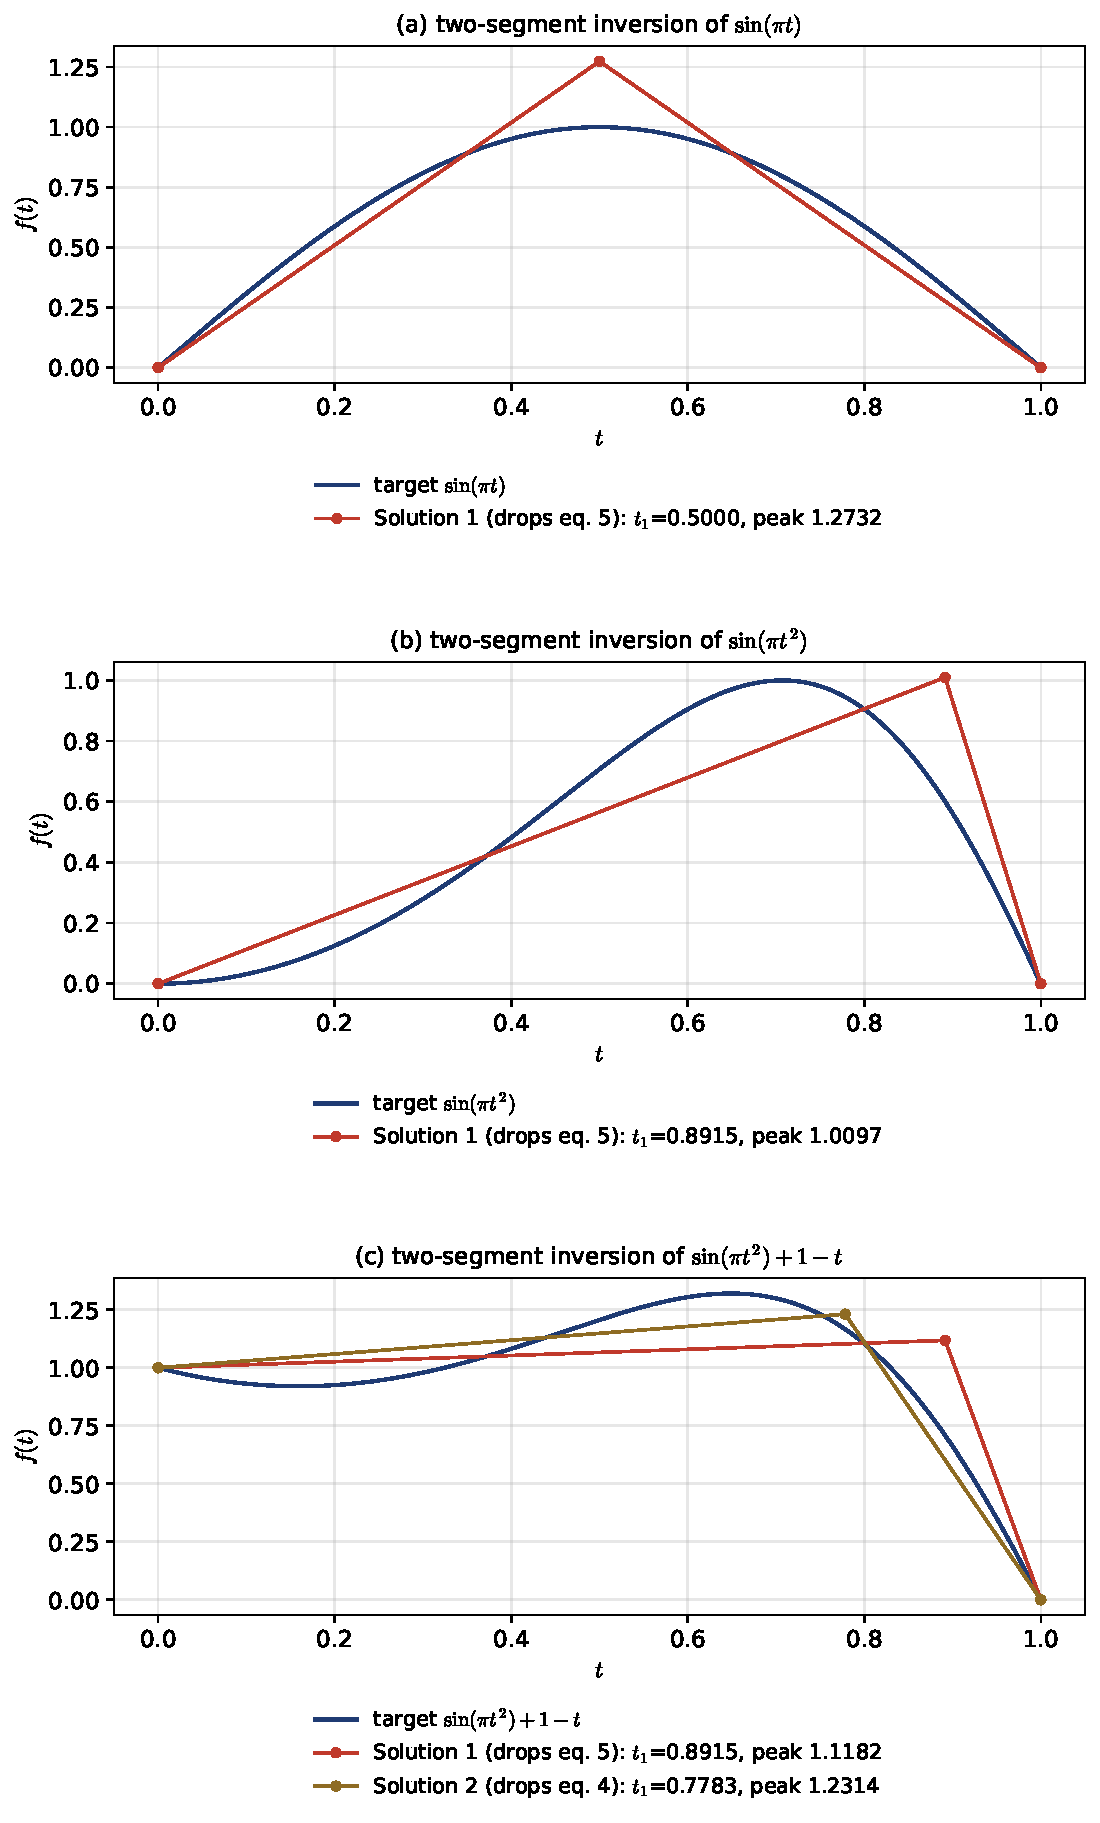
\includegraphics[width=0.7\linewidth]{_figs/fig4_two_piece}
\caption{Two-segment inversions (\texttt{two\_piece\_inversion} in \texttt{coresig.py}). (a)
$\sin(\pi t)$: Solution 1 is the symmetric tent with peak $(1/2,4/\pi)$;
Solution 2 does not exist because $z_{2}=0$. (b) $\sin(\pi t^{2})$:
Solution 1 places the peak at $t_{1}=0.8915$. (c) $\sin(\pi t^{2})+1-t$:
both solutions exist, with $t_{1}=0.8915$ and $0.7783$, and cross close
to the curve.\label{fig:twopiece}}
\end{figure}

The routine \texttt{two\_piece\_inversion} in \texttt{coresig.py}
inverts a two-segment target numerically instead of through the closed
forms of Section S2 of the supplement: the
duration is $T=z_{1}$, equations $\#2$--$\#3$ are linear in the two
slopes for a given breakpoint, and the remaining kept equation is
solved for the breakpoint by bracketing; every root is returned with
the residual of the dropped equation, which tests compatibility with the omitted coordinate.

\subsection{Adversarial cases and three pieces}


A vanishing $\Delta$ does not by itself imply failure: it gives exact
recovery when the target is a straight line. For an oscillatory target
such as $f(t)=\sin(2\pi t)$, however, the level-two coordinates agree
with the chord while higher coordinates do not. Proposition
\ref{prop:twopiece} then excludes a two-segment representation. A
third segment enlarges the candidate class without guaranteeing exact
recovery. At level four the matching system has eight equations in
six unknowns, including $T$ (Section S2 of the supplement). Dropping two equations
leaves a square system but does not guarantee an admissible solution
or satisfaction of the omitted equations. From three segments onward
we use the regression below with all retained coordinates.

\subsection{Regression over piecewise-linear paths\label{subsec:Regression}}

For four or more segments the algebraic Gröbner approach becomes prohibitively
expensive. The practical alternative is a nonlinear weighted least-squares
regression in signature space: with $\theta$ parameterising the piecewise-linear
path and $\mathcal{L}_{m}$ the set of Lyndon words up to level $m$,
\begin{equation}
\theta^{\star}\;=\;\underset{\theta}{\arg\min}\;\sum_{w\in\mathcal{L}_{m}}w_{w}\bigl(\sigma_{w}[g_{\theta}]-\sigma_{w}[X]\bigr)^{2}\,.\label{eq:weighted-regression}
\end{equation}

The experiments use level-only weights $w_w=W_{|w|}$. Table
\ref{tab:weights} compares the hand-chosen schedule
$\{50,50,30,10,10,3,3,3\}$, target-magnitude normalisation and
uniform weights. The magnitude schedule is used in the other
numerical illustrations. For a path of total variation $V$, the
factorial bound $|\sigma_w|\le V^{|w|}/|w|!$ motivates attention
to scaling, but does not determine statistically optimal weights.

For a theoretical constrained problem, one may require durations
$\Delta t_i\ge\delta>0$, $n\delta\le T$, and slopes
$|\beta_i|\le B$. This gives a compact parameter set. The signature
map and its weighted residual are continuous, so a minimiser exists
on this set; neither uniqueness nor successful recovery by a local
solver follows from that argument.

The routine \texttt{weighted\_regression} in \texttt{coresig.py} solves
a related penalised problem. Its
$2n-1$ parameters are the interior breakpoints and slopes; a finite
penalty discourages durations below \texttt{dt\_min}, and the slopes
and individual knots have bounds; the penalty is finite, so short
durations are discouraged, not excluded. SciPy's bounded trust-region
reflective solver is run from several initial points; the routine
reports the starts that meet its stopping criteria and returns the
lowest-cost result found, and meeting those criteria does not certify
a local minimum. The function name
\texttt{variance\_equalising\_weights} is retained in the code for
compatibility with earlier runs; it implements the
magnitude schedule defined in Section \ref{subsec:Weights}.

Figure \ref{fig:sinpaths4pts} shows four- and five-segment fits to
two oscillatory time-ordered paths; Figure \ref{fig:digit5_5} takes
the regression to two paths that are not time-ordered.

\begin{figure}[H]
\centering
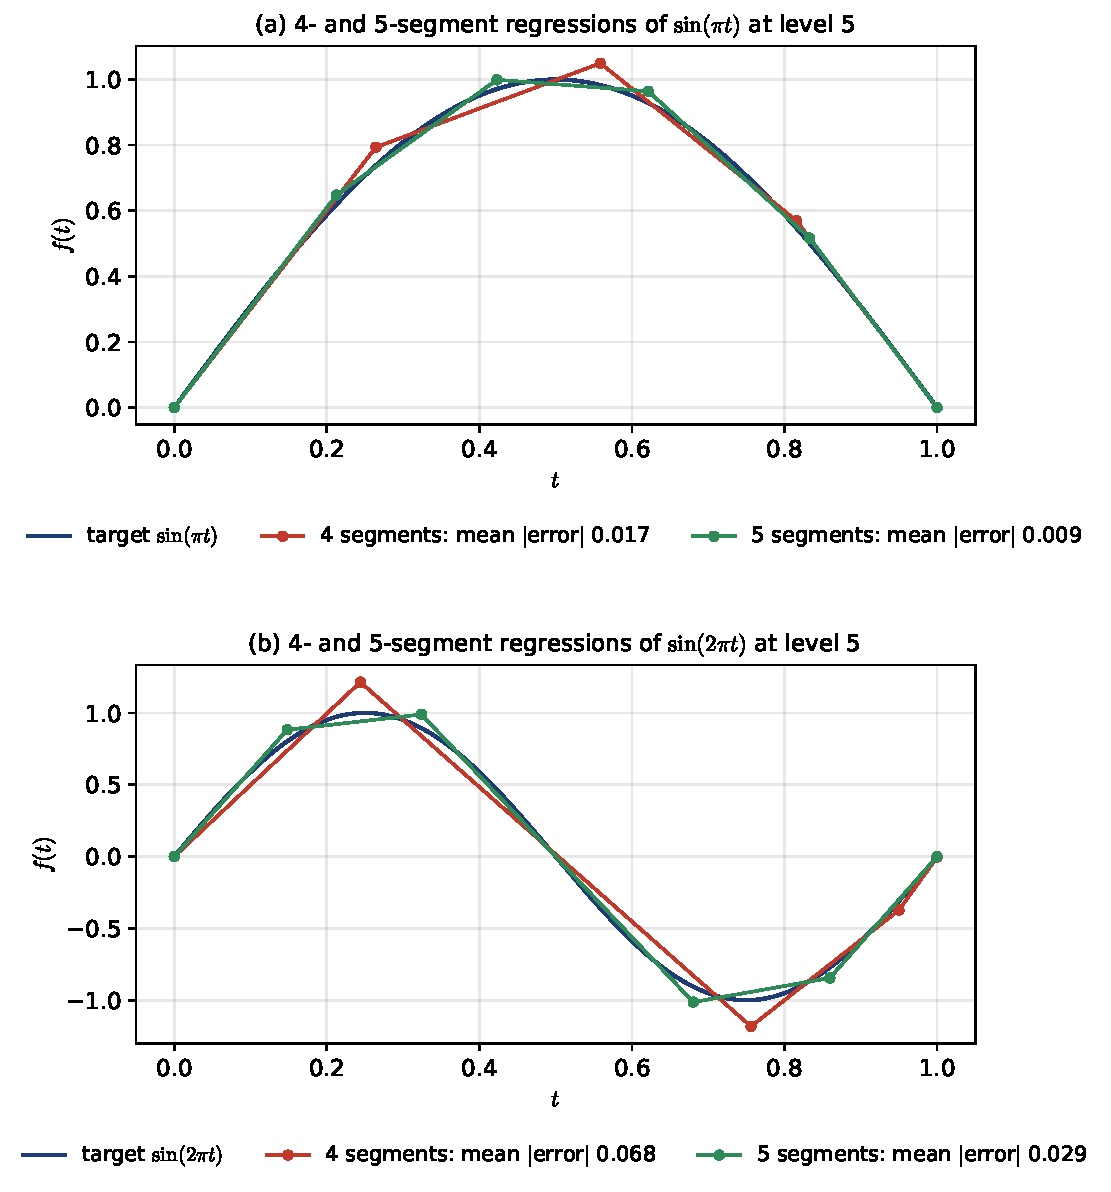
\includegraphics[width=0.92\linewidth]{_figs/fig4_multi_piece}
\caption{Four- and five-segment regressions (\texttt{weighted\_regression})
at level 5 with magnitude-normalised weights, 24 starts. (a) $\sin(\pi t)$:
mean absolute error 0.017 with four segments, 0.009 with five. (b)
$\sin(2\pi t)$: 0.068 and 0.029; one full period asks for more than
four segments, and the four-segment fit puts a breakpoint at the
minimum-duration penalty threshold.\label{fig:sinpaths4pts}}
\end{figure}

General two-dimensional paths, with the knots free in both
coordinates, use the same regression with $2(n-1)$ unknowns; with the
starting point at the origin, the level-1 entries fix the endpoint.
The routine \texttt{weighted\_regression\_2d} matches the planar
signature of the ordered vertices, and segment durations do not enter
its objective. Without a clock coordinate the entries are no longer
moments, and the semicircle and the digit 5 illustrate inversion in
this planar formulation. On the semicircle, the five-segment regression at level 5
finds a self-crossing polygon, 1.96 chords long, with a near-retracing
at the top of the arc, whose core entries match the arc's to a residual
of $5\times10^{-7}$, three hundred times smaller than the near-arc
solution's; exact out-and-back excursions cancel at every level
(Proposition \ref{prop:retracing}), and the near-retracing in this fit
comes with a small finite-level residual. Adding
one residual, a small multiple of the path length in excess of the
chord (coefficient 0.03 in the units of the weighted residuals),
penalises longer polygons and yields a fit following the arc in this
experiment (Figure \ref{fig:digit5_5}): five
segments within 0.047 of the arc, length 1.60 chords against the arc's
1.57. The digit-5 fit uses the same planar objective (Figure
\ref{fig:digit5_5}b). A clock-dependent inversion retains a chosen
clock as an additional coordinate --- arc length, interpolated vertex
index, or a spatial coordinate that is strictly monotone along the
traversal --- and its mixed entries can change the fitted polygon; the
present planar fits use spatial entries only. The next results concern
identification and stability for paths with a specified time
coordinate.

\begin{figure}[htbp]
\centering
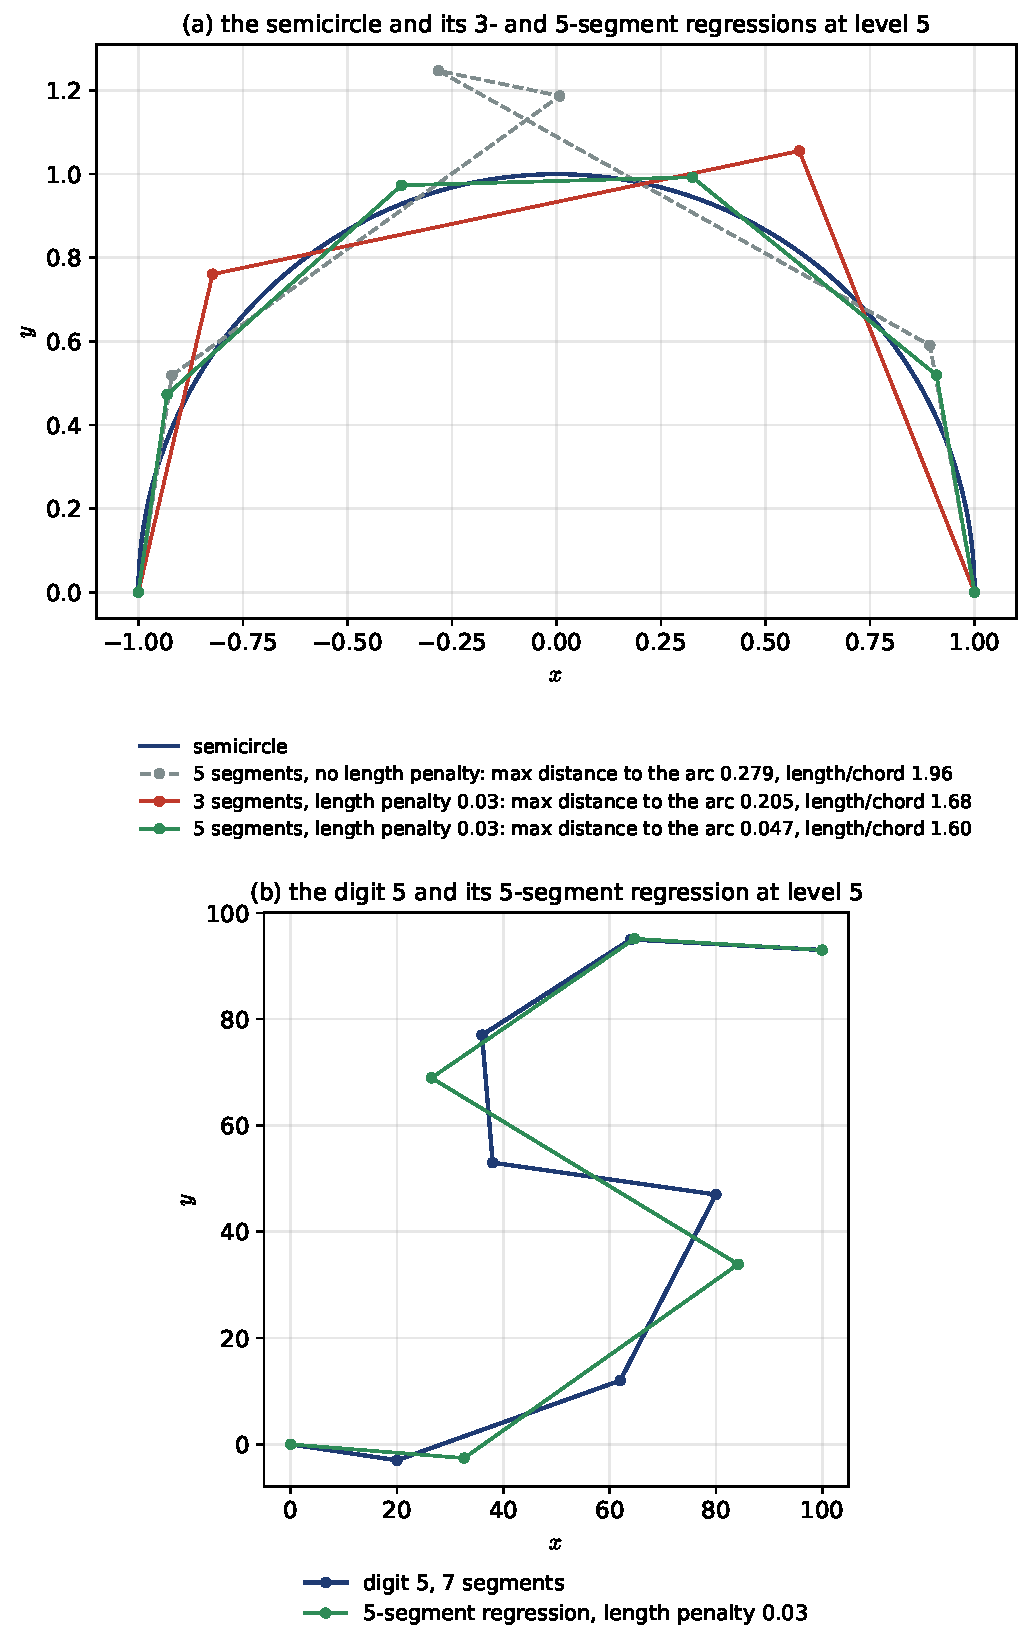
\includegraphics[width=0.75\linewidth]{_figs/fig4_general_2d}
\caption{General two-dimensional paths. (a) The semicircle and its
regressions at level 5, magnitude-normalised weights, 24 starts: five
segments without the length penalty (grey, dashed) is the self-crossing
polygon with the smallest signature residual, 1.96 chords long, with a
near-retracing at the top; three and five segments with the penalty
follow the arc, the five-segment one within 0.047 and 1.60 chords long
against the arc's 1.57.
(b) A seven-segment path tracing the digit 5 (knots in the repository
file \texttt{digit5\_points.csv}) and its five-segment regression with
the penalty, which recovers the topology of the
stroke.\label{fig:digit5_5}}
\end{figure}

\subsection{Signature entries as iterated path moments}

For $X(t)=(t,f(t))$ on $[0,T]$ with $f$ absolutely continuous, write
$M_{k}(f)=\int_{0}^{T}t^{k}f(t)\,dt$ for the moments of $f$ and $F(t)=\int_{0}^{t}f$.
The core entries of $X$ split into two families: the words $(1^{k-1},2)$
with a single letter 2, and the words with two or more.

\begin{proposition}[Single-letter-2 entries are the moments of $df$]
\label{prop:moment-identity}
For every $k\geq1$,
\[
\sigma_{(1^{k-1},2)}[X]\;=\;\frac{1}{(k-1)!}\int_{0}^{T}t^{k-1}\,df(t)\;=\;\frac{T^{k-1}}{(k-1)!}\,f(T)\;-\;\frac{M_{k-2}(f)}{(k-2)!}\quad(k\geq2)\,.
\]
In particular $\sigma_{2}[X]=f(T)-f(0)$, $\sigma_{1,2}[X]=Tf(T)-M_{0}(f)$
and $\sigma_{1,1,2}[X]=\tfrac{T^{2}}{2}f(T)-M_{1}(f)$.
\end{proposition}

\begin{proof}
The iterated integral over $0<t_{1}<\cdots<t_{k-1}<t_{k}<T$ of $dt_{1}\cdots dt_{k-1}\,df(t_{k})$
integrates the first $k-1$ variables to $t_{k}^{\,k-1}/(k-1)!$. Integration
by parts against $df$ gives the boundary term (the $t=0$ term vanishes
for $k\geq2$) minus $\int_{0}^{T}t^{k-2}f\,dt/(k-2)!$.
\end{proof}

\begin{corollary}[$D$ levels recover a degree-$D$ curve]
\label{cor:hilbert}
Let $f(t)=\sum_{i=1}^{D}\alpha_{i}t^{i}$ on $[0,1]$. The $D$ entries
$\sigma_{(1^{l-1},2)}[X]$, $l=1,\ldots,D$, determine $\alpha$ by one
linear solve: $\sigma_{(1^{l-1},2)}=\frac{1}{(l-1)!}\sum_{i}\alpha_{i}\,\frac{i}{l+i-1}$,
and the matrix $\bigl(i/(l+i-1)\bigr)_{l,i}$ is nonsingular.
\end{corollary}

\begin{proof}
$\int_{0}^{1}t^{l-1}\,d(t^{i})=i\int_{0}^{1}t^{l+i-2}\,dt=i/(l+i-1)$.
The matrix is the Hilbert matrix $\bigl(1/(l+i-1)\bigr)$ with column
$i$ scaled by $i$; the Hilbert matrix is nonsingular (it is a Cauchy
matrix), and column scaling preserves that.
\end{proof}


This is recovery within a specified polynomial family; a parameter
count alone gives no corresponding theorem for another family.
Conditioning also matters. At $D=5$, the column-scaled Hilbert matrix
in the corollary has condition number about $2.8\times10^5$, compared
with $4.8\times10^5$ for the Hilbert matrix. The unscaled signature
map includes factorial row factors and can be worse conditioned.
Additional core entries provide additional residuals; whether they
improve conditioning or lower the recovery depth is a property of the
family, treated in Theorem \ref{thm:localdepth}.

On a polynomial family the moment map also gives a stability
statement at a fixed level, which is separate from the infinite-dimensional question at the end of
Section \ref{subsec:Weights}.

\begin{theorem}[Finite-level stability on polynomial families]
\label{thm:polystab}
Fix $T>0$, an integer $D\geq1$, an exponent $s\geq0$ and positive
weights $q_{w}$ for the Lyndon words $w$ of length at most $D$. Let
$\mathcal{P}_{D}^{0}$ be the polynomials of degree at most $D$ with
$f(0)=0$, let $K\subset\mathcal{P}_{D}^{0}$ be bounded, and for
$f,g\in\mathcal{P}_{D}^{0}$ put
\[
E_{D}(f,g)\;=\;\sum_{|w|\leq D,\,w\in\mathcal{L}}q_{w}\bigl(\sigma_{w}[X_{f}]-\sigma_{w}[X_{g}]\bigr)^{2}\,,\qquad X_{f}=(t,f(t))\,.
\]
Then there are constants $0<c\leq C<\infty$, depending on $D$, $T$,
$s$, the weights and (for $C$) the size of $K$, such that
\[
c\,\|f-g\|_{H^{s}(0,T)}^{2}\;\leq\;E_{D}(f,g)\;\leq\;C\,\|f-g\|_{H^{s}(0,T)}^{2}\qquad\text{for all }f,g\in K\,.
\]
The constant $c$ can be chosen independently of $K$.
\end{theorem}

\begin{proof}[Sketch]
The $D$ single-letter-2 coordinates are $M\alpha$ with $M$ the scaled
Hilbert matrix of Corollary \ref{cor:hilbert}, invertible, which gives
a positive lower bound in coefficient norm,
$E_{D}(f,g)\geq q_{\min}s_{\min}(M)^{2}\|\alpha-\alpha'\|^{2}$; every
other retained coordinate is a polynomial in $\alpha$, so the
mean-value inequality on a ball containing $K$ gives an upper bound in
the same norm; and on the finite-dimensional space
$\mathcal{P}_{D}^{0}$ the coefficient norm and the $H^{s}$ norm are
equivalent, which converts both bounds into the stated ones (the
constants $c$, $C$ below include that conversion). The full proof is
in Section S4 of the supplement.
\end{proof}

The theorem is a finite-dimensional consequence of the moment map; its
value is the statement with its hypotheses, not the mechanism. The
displayed lower bound can deteriorate with $D$ through $s_{\min}(M)$, which is
$3.9\times10^{-3}$ at $D=3$ and $1.2\times10^{-6}$ at $D=5$ for $T=1$
(the $1/(l-1)!$ row scaling makes $M$ worse conditioned than the matrix
of Corollary \ref{cor:hilbert}), and target-dependent weights such as
\eqref{eq:variance-equalising} are covered only where they admit
uniform positive lower and finite upper bounds on $K$.


The constants can be specified in coefficient coordinates. Let
$H_s$ be the Gram matrix of $t,t^2,\ldots,t^D$ for the chosen
$H^s(0,T)$ inner product, let $Q$ contain the weights of the $D$
moment coordinates, and let $\Psi(\alpha)$ be the full vector of
weighted core entries $\sqrt{q_w}\sigma_w[X_f]$. On a convex closed
coefficient ball $B_R$ containing $K$, valid choices are
\[
c=\lambda_{\min}\!\left(H_s^{-1/2}M^\top QM H_s^{-1/2}\right),
\qquad
C=\sup_{\alpha\in B_R}
\left\|D\Psi(\alpha)H_s^{-1/2}\right\|_{\mathrm{op}}^2.
\]
The first follows from the moment subvector; the second follows by
integrating the derivative along a coefficient line segment. These
formulas expose dependence on the norm, degree, weights and parameter
range. They are not uniform-in-degree estimates.

\begin{corollary}[What stability gives a regression]
\label{cor:regression-bound}
Under the hypotheses of Theorem \ref{thm:polystab}, let $f\in K$ and
let $A\subset K$ be a nonempty candidate class. If $\hat{g}\in A$
satisfies $E_{D}(f,\hat{g})\leq\inf_{g\in A}E_{D}(f,g)+\varepsilon$,
then
\[
\|f-\hat{g}\|_{H^{s}}^{2}\;\leq\;\frac{C}{c}\,\inf_{g\in A}\|f-g\|_{H^{s}}^{2}+\frac{\varepsilon}{c}\,.
\]
\end{corollary}

\begin{proof}
$c\|f-\hat{g}\|^{2}\leq E_{D}(f,\hat{g})\leq E_{D}(f,g)+\varepsilon\leq C\|f-g\|^{2}+\varepsilon$
for every $g\in A$; take the infimum over $g$.
\end{proof}

The bound separates the representation error of the class, the
stability ratio $C/c$ and the optimisation gap $\varepsilon$, and says
nothing about the minimisers coinciding. It applies inside one
polynomial family; it does not cover the piecewise-linear fits of
Sections \ref{subsec:Regression} and \ref{sec:Curves}, and a
multi-start search does not certify a gap $\varepsilon$.


\begin{theorem}[Local identification and stability]
\label{thm:localdepth}
Let $\theta\mapsto f_\theta$ be an anchored family indexed by an open
set $\Theta\subset\mathbb R^p$. Suppose every core coordinate is
$C^1$ in $\theta$, and the vector $S_m(\theta)$ of coordinates
through level $m$ has Jacobian of rank $p$ at $\theta_0$.
Then some $p$ of these coordinates define a $C^1$ diffeomorphism
from a neighbourhood $U$ of $\theta_0$ onto an open set. Every other
core coordinate is a $C^1$ function of the selected coordinates on
$U$. After reducing $U$, there are $a,b>0$ such that
\[
a|\theta-\eta|\le |S_m(\theta)-S_m(\eta)|
\le b|\theta-\eta|\qquad(\theta,\eta\in U).
\]
If, additionally, $\theta\mapsto f_\theta$ is $C^1$ into a chosen
$H^s(0,T)$ space with injective derivative at $\theta_0$, the
parameter distance in this estimate can be replaced by
$\|f_\theta-f_\eta\|_{H^s}$, with different constants.
\end{theorem}

\begin{proof}[Sketch]
Apply the inverse function theorem to an invertible $p$-row minor $F$
of $DS_{m}(\theta_{0})$; every other coordinate factors through
$F^{-1}$. On a small convex ball the variation of $DF$ is below half
the smallest singular value of $DF(\theta_{0})$, and integrating
derivatives along segments gives the two-sided estimate; the $H^{s}$
version uses the injectivity of the path derivative. The full proof
is in Section S4 of the supplement.
\end{proof}

For a fixed parameterisation, define its local identification depth
at a point as the smallest $m$ satisfying this rank condition, when
such an $m$ exists. Redundant parameters must first be removed. The
theorem is local and conditional: it does not supply a rank condition
from a parameter count, or prove global identifiability. Higher
coordinates are locally redundant for exact identification but may
remain useful for estimation with noise.

\begin{remark}[Entries with more than one letter 2; the depth of a curve]
\label{rem:nonlinear-core}
Lyndon words with two or more letter 2s are iterated integrals of $f$
against itself, and are not determined by the finitely many moments
retained at a given level (the full moment sequence determines $f$ on
a compact interval, and with it every entry); for instance
\[
\sigma_{1,2,2}[X]=\int_{0}^{T}\Bigl(\int_{0}^{u}t\,df(t)\Bigr)df(u)=\frac{T}{2}f(T)^{2}+\frac{1}{2}\int_{0}^{T}f^{2}-f(T)\,F(T)\,,
\]

which depends on $\int f^2$. On a fixed finite-dimensional family,
such coordinates can contribute to the rank of the signature map.
Whether they reduce identification depth must be checked for that
family. A Nelson--Siegel--Svensson curve has an additive level
parameter invisible to the signature. After fixing that level,
five shape parameters remain; the numerical rank-five moment
Jacobians found at three parameter sets are local evidence at those
points; generic rank, and the behaviour at degenerate decay parameters
or vanishing loadings, remain to be established. Theorem
\ref{thm:localdepth} states what a verified rank condition gives. The
market interpolants in Section \ref{sec:Curves} belong to no named
family; their fit-error sweep tests a numerical choice of truncation.

\end{remark}


Recovering a function from finitely many moments is an inverse
problem with substantial conditioning difficulties \cite{Talenti}.
The first $m$ moments of $f$ determine its $L^2$ projection onto
polynomials of degree below $m$. For an integer $r\ge1$ and
$f\in C^r([0,T])$, polynomial approximation estimates imply an
$O(m^{-r})$ error for that projection in $L^2$
\cite[Chapter 7]{DeVoreLorentz}. This is an approximation result for
polynomials of increasing degree, not a rate for a fixed-segment
signature regression. Matching increment moments also fixes ordinary
moments only after the relevant endpoint increment is matched and
the initial value is fixed.

\paragraph{Path-space evaluation.}
A signature residual and a path-space error measure different
quantities. For time-ordered paths, a direct numerical benchmark is
to minimise
\[
\frac{1}{N+1}\sum_{i=0}^{N}|f(t_i)-g_\theta(t_i)|,
\qquad t_i=iT/N,
\]
over the same candidate class and constraints. This is a sampled
mean absolute error, approximating $T^{-1}\|f-g_\theta\|_{L^1}$
as the grid is refined. A numerical search supplies a benchmark; the
best value it finds is an upper bound on the minimum. Corollary
\ref{cor:regression-bound} provides an approximation-quality
comparison only on the polynomial classes covered by its hypotheses.
No equality of minimisers is claimed for the piecewise-linear
experiments.

\subsection{Weights, and what the regression minimises\label{subsec:Weights}}


\paragraph{Target-magnitude normalisation.}
For each level, let $a_l$ be the largest absolute target \emph{core}
coordinate at that level. The implemented schedule is
\begin{equation}
a_l=\max_{\substack{w\in\mathcal L_m\\|w|=l}}|\sigma_w[X]|,
\quad A=\max_{w\in\mathcal L_m}
\bigl(|w|!\,|\sigma_w[X]|\bigr)^{1/|w|},
\quad \widetilde W_l=\frac{1}{\max(a_l,0.1A^l/l!)^2},
\quad W_l=\frac{\widetilde W_l}{\widetilde W_1}.
\label{eq:variance-equalising}
\end{equation}
The floor prevents a vanishing level from receiving an infinite
weight. The time coordinate ensures $A>0$ in the time-ordered
experiments. This schedule scales residuals relative to target
magnitudes; it is not a derived residual covariance. It also need
not equalise contributions from different levels, which have
different numbers of core coordinates. Changing $m$ can change $A$
and hence weights at earlier levels where the floor is active.
The working and uniform schedules in Table \ref{tab:weights} provide
comparators. None of these numerical comparisons establishes an
optimal schedule for a general noise model.

For contrast, the following calculation gives inverse marginal
variances under a specific stochastic model.

\begin{proposition}[Brownian-bridge moment variances]
\label{prop:bridge}
Let $B$ be a standard Brownian bridge on $[0,1]$ and $X=(t,B)$. For
$l\geq2$,
\begin{align*}
\mathrm{Var}\,\sigma_{(1^{l-1},2)}[X] & =\frac{1}{((l-2)!)^{2}\,l^{2}\,(2l-1)}\,,\\
W_{l}^{\mathrm{bridge}}:=\frac{1}{\mathrm{Var}\,\sigma_{(1^{l-1},2)}} & =12,\;45,\;448,\;8100,\;\ldots\;\sim\;\frac{2\,(l!)^{2}}{l}\,.
\end{align*}
\end{proposition}

\begin{proof}
The bridge has unbounded variation; the single-letter-2 entries
$\frac{1}{(l-1)!}\int_{0}^{1}t^{l-1}\,dB_{t}$ have deterministic
integrands and are Wiener integrals, for which integration by parts
holds as for Proposition \ref{prop:moment-identity}. With $B_{0}=B_{1}=0$,
$\sigma_{(1^{l-1},2)}=-\frac{1}{(l-2)!}\int_{0}^{1}t^{l-2}B_{t}\,dt$.
With $a=l-2$ and $\mathrm{Cov}(B_{s},B_{t})=\min(s,t)-st$, the double
integral of $s^{a}t^{a}(\min(s,t)-st)$ over $[0,1]^{2}$ is
$\frac{2}{(a+2)(2a+3)}-\frac{1}{(a+2)^{2}}=\frac{1}{(a+2)^{2}(2a+3)}$,
and $(a+2)^{2}(2a+3)=l^{2}(2l-1)$. Stirling's formula gives the asymptotic.
\end{proof}


The inverse marginal variances grow factorially, with the additional
factor $2/l$ shown above. This calculation concerns one coordinate
per level and does not identify the covariance of all core residuals.
Nor are these moment coordinates independent, as the next result
shows. The distinction matters when interpreting weighted least
squares \cite{Aitken}.

\begin{proposition}[Bridge covariance of the moment coordinates]
\label{prop:bridgecov}
With $B$ and $Z_{l}:=\sigma_{(1^{l-1},2)}[(t,B)]$ as in Proposition
\ref{prop:bridge}, for $r,s\geq2$,
\[
\mathrm{Cov}(Z_{r},Z_{s})\;=\;\frac{1}{(r-1)!\,(s-1)!}\Bigl(\frac{1}{r+s-1}-\frac{1}{rs}\Bigr)\,.
\]
For every $m\geq2$ the covariance matrix of $(Z_{2},\ldots,Z_{m})$ is
positive definite. If a curve is observed as $f+\varepsilon B$, the
perturbations of its moment coordinates are exactly $\varepsilon Z_{l}$,
so their covariance is $\varepsilon^{2}$ times this matrix, and the
covariance-weighted residual on the moment coordinates is the
generalised least-squares objective for that family under that model.
\end{proposition}

\begin{proof}
Write $B_{t}=W_{t}-tW_{1}$ with $W$ a Brownian motion. Then
$Z_{l}=\frac{1}{(l-1)!}\int_{0}^{1}(t^{l-1}-\tfrac{1}{l})\,dW_{t}$,
since $\int_{0}^{1}t^{l-1}\,d(tW_{1})=W_{1}/l$, and the It\^{o} isometry
gives $\mathrm{Cov}(Z_{r},Z_{s})=\frac{1}{(r-1)!(s-1)!}\int_{0}^{1}(t^{r-1}-\tfrac{1}{r})(t^{s-1}-\tfrac{1}{s})\,dt$,
which is the formula; the diagonal is Proposition \ref{prop:bridge}.
The matrix is the Gram matrix of the functions $t^{l-1}-1/l$,
$l=2,\ldots,m$, in $L^{2}(0,1)$, scaled by nonzero factorials; these
functions are linearly independent (distinct degrees), so the Gram
matrix is positive definite. The last statement is the linearity of
$\sigma_{(1^{l-1},2)}$ in $df$ (Proposition \ref{prop:moment-identity}).
\end{proof}

The off-diagonal entries are large: $\mathrm{Corr}(Z_{2},Z_{3})=\sqrt{15}/4$.
So under the bridge model the justified objective on the moment
coordinates is the quadratic form of the inverse covariance, and the
diagonal weights of Proposition \ref{prop:bridge} are its marginals
only. The proposition says nothing about the entries with more than
one letter 2, which are nonlinear in the path, nor about the level-1
entry, which the bridge leaves unchanged and which must be treated separately.
A covariance calculation for the nonlinear coordinates requires an
integration convention and further analysis; the schedule \eqref{eq:variance-equalising} used in the
experiments remains a magnitude normalisation.


\paragraph{Does the schedule matter?}
Table \ref{tab:weights} reports errors that the signature objective
does not directly minimise. For the six smooth-function configurations,
the mean absolute errors differ by less than 5\% across schedules;
maximum errors differ by up to about 10\%. This does not imply that
the fitted polygons or their breakpoints coincide. On DI1 the
magnitude schedule reduces the maximum error from 14.8 bp under
the working weights to 6.5 bp; uniform weights give 6.9 bp.
On the Treasury curve the magnitude schedule gives 10.4 bp,
compared with 9.2 and 9.3 bp for the other schedules.

Termination counts also depend on the schedule. Magnitude
normalisation has the largest counts on the two curves and on
$\sin(2\pi t)$, while it has the smallest counts on
$\sin(\pi t^2)$. These are outcomes of a twelve-start experiment.
Weighting changes the objective as well as its numerical scaling.

\begin{table}[H]
\centering
\small
\begin{tabular}{@{}lr rrr rrr rrr@{}}
\toprule
Target & $n$ & \multicolumn{3}{c}{mean $|$error$|$} & \multicolumn{3}{c}{max $|$error$|$} & \multicolumn{3}{c}{starts converged (of 12)} \\
\cmidrule(lr){3-5}\cmidrule(lr){6-8}\cmidrule(lr){9-11}
 & & work. & magn. & unif. & work. & magn. & unif. & work. & magn. & unif. \\
\midrule
$\sin(\pi t)$ & 4 & 0.0161 & 0.0168 & 0.0161 & 0.0657 & 0.0647 & 0.0659 & 5 & 5 & 4 \\
$\sin(\pi t)$ & 5 & 0.0093 & 0.0093 & 0.0092 & 0.0340 & 0.0351 & 0.0339 & 3 & 6 & 3 \\
$\sin(2\pi t)$ & 4 & 0.0670 & 0.0694 & 0.0670 & 0.2302 & 0.2095 & 0.2259 & 6 & 10 & 4 \\
$\sin(2\pi t)$ & 5 & 0.0292 & 0.0292 & 0.0292 & 0.1032 & 0.1059 & 0.1036 & 4 & 8 & 7 \\
$\sin(\pi t^{2})$ & 4 & 0.0179 & 0.0181 & 0.0178 & 0.0740 & 0.0708 & 0.0730 & 9 & 7 & 10 \\
$\sin(\pi t^{2})$ & 5 & 0.0123 & 0.0126 & 0.0123 & 0.0423 & 0.0403 & 0.0425 & 5 & 4 & 6 \\
DI1 (bp) & 5 & 3.9 & 1.9 & 2.2 & 14.8 & 6.5 & 6.9 & 2 & 6 & 2 \\
H.15 (bp) & 4 & 3.9 & 4.2 & 3.9 & 9.2 & 10.4 & 9.3 & 4 & 11 & 5 \\
\bottomrule
\end{tabular}
\caption{Three weight schedules, level 5, twelve starts, segment-duration
penalty threshold 2\%: the working values $\{50,50,30,10,10,3,3,3\}$,
the magnitude weights \eqref{eq:variance-equalising}, and uniform weights. Pointwise
error on a 401-point grid for the functions (units of the target), at
the market points for the curves (bp); breakpoints and costs in the
repository file \texttt{weights\_comparison.csv}.\label{tab:weights}}
\end{table}




\paragraph{An all-level metric and its limits.}
Finite-level norm equivalence on a specified polynomial space does
not pass automatically to an infinite-dimensional class.

\begin{proposition}[An obstruction to undamped weighting]
\label{prop:obstruction}
Let $W_k>0$ satisfy $\sum_{k\ge2}W_k/(k!)^2=\infty$.
Then the weighted squared core difference over all levels diverges
between $X=(t,0)$ and either $G=(t,at)$ or $G=(t,at(1-t))$ on
$[0,1]$, for $a\ne0$. The second pair has identical endpoints.
\end{proposition}

\begin{proof}
The single-letter-2 differences are $a/k!$ for $g(t)=at$ and
$a(1-k)/((k+1)k!)$ for $g(t)=at(1-t)$. Summing their weighted squares
proves the first assertion directly. In the second case the factor
$(k-1)^2/(k+1)^2$ tends to one, giving the same conclusion.
\end{proof}

This covers weights proportional to $(k!)^2$ and also the inverse
bridge variances, for which $W_k/(k!)^2\sim2/k$. The obstruction is
finiteness, before any question of a Sobolev lower bound. Damping
the weights gives a well-defined distance with a qualitative
recovery guarantee.

\begin{theorem}[A damped core metric on a Lipschitz class]
\label{thm:dampedmetric}
Fix $T>0$, $L>0$, set $A=\max(1,L)$, and let
\[
K_L=\{f\in C([0,T]):f(0)=0,\ |f(t)-f(u)|\le L|t-u|\}.
\]
For $0<\rho<1/(\sqrt2 A)$, define
\[
d_\rho(f,g)^2=
\sum_{w\in\mathcal L}
\frac{(|w|!)^2\rho^{2|w|}}{T^{2|w|}}
|\sigma_w[(t,f)]-\sigma_w[(t,g)]|^2.
\]
This series converges uniformly on $K_L\times K_L$. Its square
root is a metric on $K_L$ and induces the uniform topology.
In particular, there is a nondecreasing function $\omega$ with
$\omega(r)\to0$ as $r\downarrow0$ such that
\[
\|f-g\|_\infty\le\omega(d_\rho(f,g))\qquad(f,g\in K_L).
\]
\end{theorem}

\begin{proof}[Sketch]
Simplex integration gives $|\sigma_{w}|\le A^{k}T^{k}/k!$ for a word
of length $k$, so the level-$k$ weighted squared differences are at
most $4(2A^{2}\rho^{2})^{k}$ and the series converges; $d_{\rho}$ is
an $\ell^{2}$ norm of a difference, hence a metric, and
$d_{\rho}(f,g)=0$ forces all moments of $f-g$ to vanish (Proposition
\ref{prop:moment-identity}), so $f=g$. Each iterated integral is
continuous for uniform convergence under a common variation bound, by
induction on the word length; $K_{L}$ is compact by
Arzel\`a--Ascoli, so the continuous injection is a homeomorphism onto
its image and its inverse is uniformly continuous. The full proof is
in Section S4 of the supplement.
\end{proof}

The theorem establishes topological recovery on a fixed compact
class; a Lipschitz or H\"older inverse, a Sobolev norm equivalence,
and a bound uniform in $L$ are the stronger statements that remain
open on an infinite-dimensional class.

\paragraph{Open questions.}
For the metric above, determine quantitative bounds on the inverse
modulus $\omega$, and identify additional assumptions under which
an inverse estimate in a specified path norm holds. For finite-level
piecewise-linear recovery, determine the parameter domains and
levels on which a full-rank Jacobian gives useful stability
constants, accounting for coincident slopes and collapsing
durations. Similar numerical fits from two regression objectives are
evidence for none of these.


\paragraph{Approximation barrier.}
The rate at which a piecewise-linear approximant converges does not
improve with the level at which the signature is read:

\begin{proposition}[Approximation barrier]
\label{prop:barrier}
For $f(t)=t^{2}$ on $[0,1]$ and any piecewise-linear $g$ with $N$
pieces, continuous or not, $\int_{0}^{1}|f-g|\,dt\geq1/(16N^{2})$.
\end{proposition}

\begin{proof}
On an interval of length $h$ centred at $c$, write $t=c+x$; then
$t^{2}-(\text{affine in }t)=x^{2}-(\text{affine in }x)$, and the
best $L^{1}$ affine approximation of $x^{2}$ on $[-h/2,h/2]$ has slope
zero by symmetry (the objective is convex in the affine coefficients and
invariant under $x\mapsto-x$) and intercept equal to the median of
$x^{2}$ under the uniform law, $h^{2}/16$; its error is
$\int_{-h/2}^{h/2}|x^{2}-h^{2}/16|\,dx=h^{3}/16$. Summing over pieces
of lengths $h_{i}$ with $\sum h_{i}=1$ and using
$\sum h_{i}^{3}\geq N(1/N)^{3}$ gives the bound.
\end{proof}

Thus no rate faster than $N^{-2}$ can hold uniformly for this
piecewise-linear approximation problem on a smooth target class
containing $t^2$ (individual targets, such as affine functions, are
recovered exactly). A faster rate needs pieces of higher degree, a
different model class.


\subsection{What the estimates establish}

The results distinguish four conclusions. Lyndon coordinates remove
algebraic redundancy without discarding truncated-signature
information. Exact recovery additionally requires membership of a
specified path family's signature image. Finite-level stability
holds on the polynomial families of Theorem \ref{thm:polystab} and
locally under the hypotheses of Theorem \ref{thm:localdepth}.
The all-level metric of Theorem \ref{thm:dampedmetric} gives a
qualitative inverse modulus on a Lipschitz class. None of these
statements identifies weighted signature regression with a Sobolev
orthogonal projection, or certifies the numerical optimiser used in
the examples.

%% =========================================================================
\section{Two term structures: an illustration\label{sec:Curves}}
%% =========================================================================

This section runs the inversion of Section \ref{sec:Inversion} on one
date each of two term structures, illustrating the approximation
problem and the dependence of the fit on truncation and representation: the Brazilian one-day interbank deposit futures curve
(DI1, traded and settled at B3; settlement rates from \cite{b3data})
and the US Treasury constant-maturity curve published in the Federal
Reserve's H.15 release \cite{h15data}. The DI1 example contains 37 listed contracts extending to about
fourteen years. The Treasury example uses eleven constant-maturity
tenors and a public data source. The dates are 7 November 2023 for DI1 and
11 October 2023 for H.15, the last dates in the two data files. The code
is the Python module of Section \ref{sec:Core} and the scripts in the
repository.

\paragraph{Representation.}
A curve on a given date is the time-augmented path $X(u)=(u,x(u))$,
where $x$ is the rate in percent relative to its first value (the level
is stored separately; the signature sees only $dx$) and $u$ is the
maturity axis mapped to $[0,1]$ by $u=(\sqrt{\tau}-\sqrt{\tau_{0}})/(\sqrt{\tau_{\max}}-\sqrt{\tau_{0}})$.
The square root spreads the short end, where most of the shape lives;
its effect on the regression is discussed in Section \ref{subsec:CurveLevels}.
The target signature is that of the linear interpolant of the market
points. The weights are the magnitude-normalisation schedule
\eqref{eq:variance-equalising} computed from that signature. The
regression is the multi-start weighted least squares of Section
\ref{subsec:Regression}, with 24 random starts and a penalty threshold
of 2\% of the path for segment duration. The level $m$ is the smallest at which the system is
overdetermined, $|C_{m}|-1>2n-1$; the number of segments $n$ is
chosen from the sweep of Section \ref{subsec:CurveLevels}, which
compares $n$ and $n-1$ for each curve and stops at the count that
reduces the reported error substantially relative to the smaller count. Larger counts were not run;
the choices are illustrative.
The script \texttt{listing5\_curve.py} in the repository shows the
inversion call for one date, using the companion module and data
loader.

\subsection{The DI1 curve}

\begin{figure}[H]
\centering
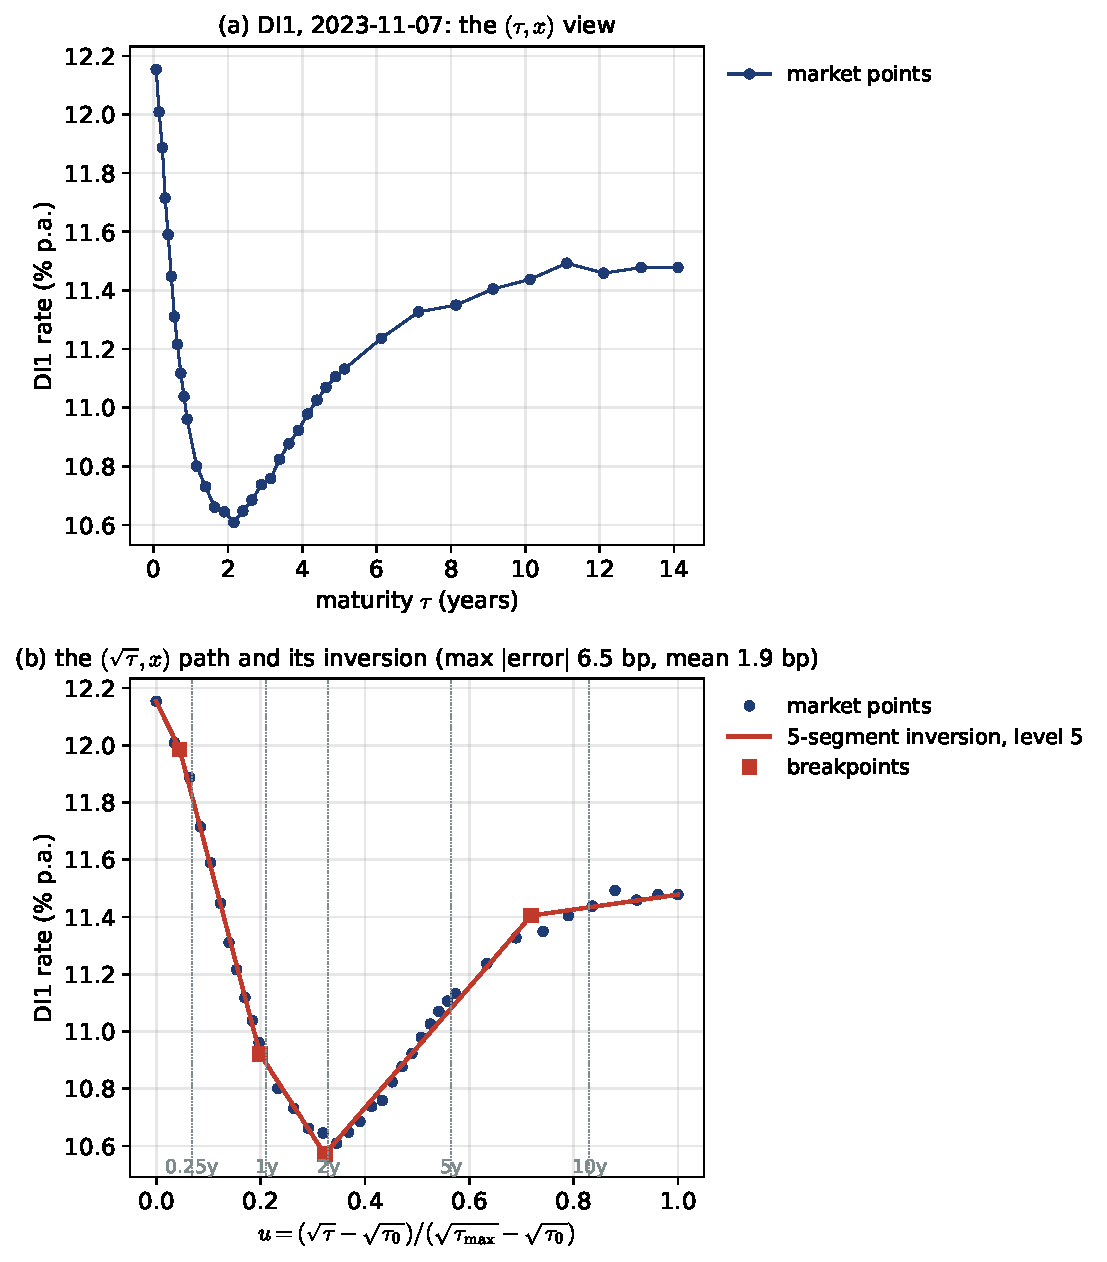
\includegraphics[width=0.92\linewidth]{_figs/fig5_di1_inversion}
\caption{DI1 futures, 7 November 2023 (37 contracts, B3 settlement
rates). (a) The curve against maturity. (b) The same curve on the
$\sqrt{\tau}$ axis with its five-segment inversion at level 5: maximum
error 6.5 bp, mean 1.9 bp at the market points; dotted lines mark
maturities.\label{fig:di1}}
\end{figure}

Figure \ref{fig:di1} shows the curve and its inversion. The five
segments place their four elbows at about 0.17, 0.91, 1.93 and 7.7 years
($u=0.045,\,0.199,\,0.323,\,0.719$). The five segments follow the
features of the curve: a steep front end to about two months, a decline to about one year,
the bottom of the trough between one and two years, a rise to nearly
eight years, and a long end that is one straight
segment in $\sqrt{\tau}$. The fit misses by at most 6.5 bp, at the 4--5 year
convexity between the third and fourth elbows, and by 1.9 bp on
average. With four segments instead of five the maximum error is 13--15
bp at level 5 and 10 bp at level 6, and the first elbow migrates to
the front of the path: the fifth segment is what gives the front end
its own piece.

\subsection{The Treasury curve}

\begin{figure}[H]
\centering
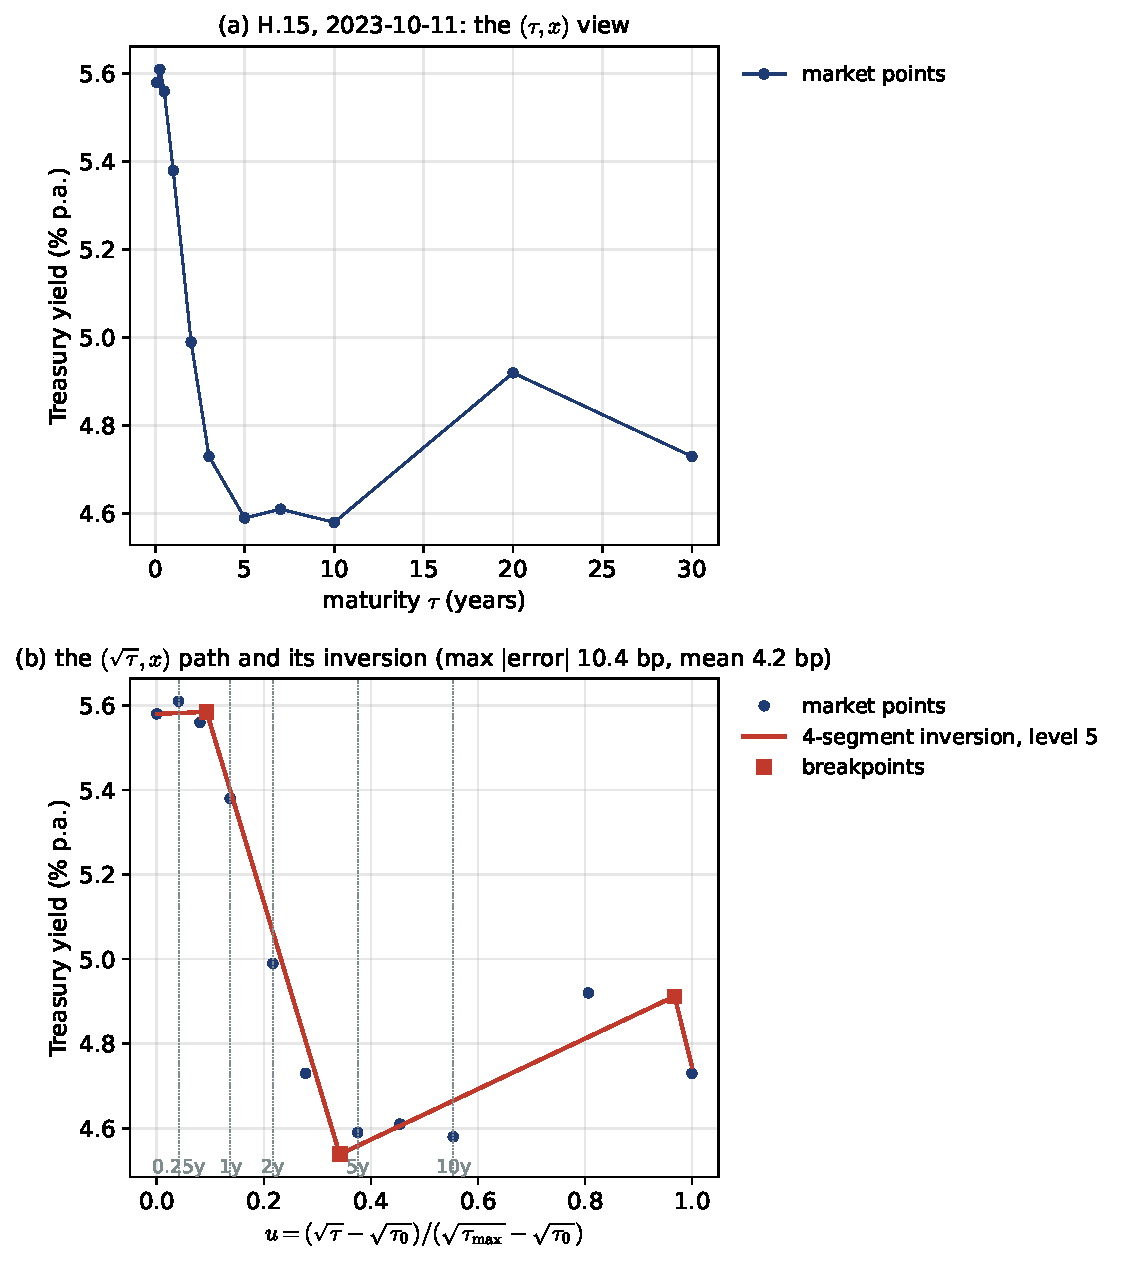
\includegraphics[width=0.92\linewidth]{_figs/fig5_h15_inversion}
\caption{US Treasury constant-maturity yields, 11 October 2023 (eleven
tenors, Federal Reserve H.15). (a) Against maturity. (b) On the
$\sqrt{\tau}$ axis with the four-segment inversion at level 5: maximum
error 10.4 bp, mean 4.2 bp.\label{fig:h15}}
\end{figure}

The Treasury curve of that date is inverted at the front, flat between
five and ten years, and humped at twenty years. Four segments at level
5 (Figure \ref{fig:h15}) place elbows at about 0.6, 4 and 28 years and
fit to 10.4 bp maximum, 4.2 bp mean. The trough is located well; the
twenty-year hump is located coarsely, the last elbow landing at 28
rather than 20 years and under-shooting the 20-year point by about 10

bp. Three segments give maximum errors of 24--27 bp at the tested
levels. For four segments, the maximum error increases from 10.4 bp
at level five to 23.0 bp at level six. The level-six magnitude weight
is about three million times the level-one weight, so changing the
truncation changes the relative emphasis of the objective strongly.
The comparison says which truncation fits this curve better; it says
nothing about what level six contains.

\subsection{Levels, segments and the maturity axis\label{subsec:CurveLevels}}

\begin{table}[H]
\centering
\begin{tabular}{@{}llrrrrl@{}}
\toprule
Curve & Date & $n$ & $m$ & max $|$err$|$ (bp) & mean $|$err$|$ (bp) & breakpoints $u$ \\
\midrule
DI1 & 2023-11-07 & 4 & 5 & 13.0 & 3.8 & 0.020, 0.273, 0.772 \\
DI1 & 2023-11-07 & 4 & 6 & 10.2 & 3.5 & 0.273, 0.367, 0.727 \\
DI1 & 2023-11-07 & 5 & 5 & \textbf{6.5} & \textbf{1.9} & 0.045, 0.199, 0.323, 0.719 \\
DI1 & 2023-11-07 & 5 & 6 & 7.5 & 2.3 & 0.078, 0.170, 0.315, 0.722 \\
\midrule
H.15 & 2023-10-11 & 3 & 4 & 25.1 & 12.3 & 0.419, 0.980 \\
H.15 & 2023-10-11 & 3 & 5 & 26.8 & 13.3 & 0.400, 0.980 \\
H.15 & 2023-10-11 & 3 & 6 & 24.9 & 13.7 & 0.393, 0.926 \\
H.15 & 2023-10-11 & 4 & 4 & 9.9 & 5.2 & (square system) \\
H.15 & 2023-10-11 & 4 & 5 & \textbf{10.4} & \textbf{4.2} & 0.093, 0.342, 0.968 \\
H.15 & 2023-10-11 & 4 & 6 & 23.0 & 13.5 & 0.383, 0.797, 0.817 \\
\bottomrule
\end{tabular}
\caption{Fit error at the market points against segments $n$ and level
$m$, magnitude-normalised weights, segment-duration penalty threshold 2\% of the path, 12--24
starts. Bold: the configurations shown in Figures \ref{fig:di1} and
\ref{fig:h15}. At level four there are seven nonconstant matching equations: fewer
than the nine parameters for $n=5$, and equal to the seven parameters
for $n=4$. These counts do not establish independence or solvability.\label{tab:sweep}}
\end{table}

Table \ref{tab:sweep} is the sweep behind the two figures. It shows
three things.


\emph{Levels.} For the selected configurations of five DI1 segments
and four Treasury segments, level five has smaller mean and maximum
errors than level six. For four DI1 segments, however, level six
improves on level five. A useful truncation therefore depends on
the target, candidate class and weighting. This sweep supplies no
rank calculation for a parameterised market-curve family and is not
an empirical verification of Theorem \ref{thm:localdepth}.

\emph{Signature error and pointwise error.} These are different
objectives. For DI1 with four segments, a 24-start search found a
lower signature residual than a 4-start search and a worse maximum
pointwise error (14.6 against 10.0 bp). The five-segment configurations reported
here fit better in path space. The table reports unweighted errors at
the market points.


\emph{The maturity axis.} On the DI1 curve the $\sqrt{\tau}$ axis
compresses the range of the magnitude-normalised weights over levels
1--6 about forty times ($2.8\times10^{6}$ under $(\tau,x)$ to
$7.2\times10^{4}$); on the Treasury curve it does not
($2.8\times10^{6}$ against $3.4\times10^{6}$), for this set of tenors
and rates. The square root changes the path, its signature and the
approximation class --- a segment straight in $\sqrt{\tau}$ is not
straight in $\tau$ --- so the best attainable fits need not coincide;
they can still be compared at common market maturities. All fitted
examples use the $\sqrt{\tau}$ axis. The weight range is a scaling
diagnostic, not a condition number of the regression Jacobian.

%% =========================================================================

\section{Conclusions}

Core signatures make the classical Lyndon-coordinate description
of a truncated signature explicit through a shuffle-elimination
procedure and substitution rules. We used these coordinates to
separate exact recovery, local identification and approximation by
weighted regression. The two-segment criterion combines an
algebraic compatibility condition with an admissible breakpoint;
the moment coordinates determine polynomial paths and yield
finite-level stability on bounded polynomial families. A rank
condition gives local parameter recovery, with a path-norm estimate
under an additional regularity assumption.

The stochastic and deterministic weighting questions have different
answers. Additive bridge noise gives an explicit covariance matrix
for the moment coordinates. The experimental magnitude schedule
instead scales entries relative to the target. For all-level
comparisons, undamped factorial growth can produce infinite
residuals; damping yields a metric inducing uniform convergence
on an anchored Lipschitz class, but does not establish a Sobolev
norm equivalence or a quantitative inverse rate. The linear-spline
approximation barrier further separates signature depth from the
expressive capacity of a candidate path class.

The DI1 and Treasury examples illustrate the numerical approximation
problem, with maximum errors of 6.5 and 10.4 bp in the selected
configurations. They show sensitivity to weighting, truncation and
the maturity representation. Quantitative stability constants
for nondegenerate piecewise-linear families and inverse-modulus
bounds for the all-level metric remain questions for further work.
The framework has been adopted in practitioner work on
quantitative-trading futuretesting; see \cite{bloch_futuretesting}.
We thank Sam Cohen (Oxford) for helpful discussions.


\paragraph{Code and data.}
The accompanying source package includes the core module, the
scripts for the displayed numerical examples, input snapshots for
the two curve dates, the digit-5 knots, and saved weight-comparison
and configuration-sweep results. Its curve loaders default to the
included snapshots. The project repository is
\url{https://github.com/MarcosCarreira/CoreSignatures}, folder
\texttt{2026 R1}; the same package accompanies the submission. The core
module uses NumPy and SciPy; the data and figure scripts additionally
use pandas and Matplotlib. The routines named in the text
(\texttt{coresig.py}) and the short scripts in \texttt{listings/} are
the code behind the displayed examples; the figure scripts reproduce
the figures from the included snapshots. The supplementary material
(rules, closed forms, and the proofs of Proposition
\ref{prop:core-is-lyndon} and of the stability theorems) is submitted
with the paper and is also in that folder.
The displayed empirical results are those of the companion runs; the
formulas and the data handling were checked separately, and the
package records those checks.

\paragraph{Use of AI assistance.}
The author used Anthropic's Claude and OpenAI's Codex to review the mathematical content
of the paper, tighten the exposition, supply the citation chain through
the Lyndon basis theorem, Poincaré--Birkhoff--Witt and Radford's theorem
that identifies the core variables with the Lyndon coordinates of
$G^{n}(\mathbb{R}^{d})$, and help write the proofs in the supplement,
the regression and weights sections, the Python module and scripts, and
the term-structure section; OpenAI's Codex was used to check
hypotheses, revise the recovery and stability statements, and check
numerical consistency. All mathematical claims, the choice of which
results to state as open problems, and the final form of the paper are
the author's responsibility.

\begingroup
\small
\begin{thebibliography}{Pfeffer, Seigal and Sturmfels (2018)}

\bibitem[Aitken (1935)]{Aitken}Aitken, A.~C.\ (1935), ``On least squares
and linear combinations of observations'', Proceedings of the Royal
Society of Edinburgh 55, 42--48,
\href{https://doi.org/10.1017/S0370164600014346}{https://doi.org/10.1017/S0370164600014346}

\bibitem[Amendola, Friz and Sturmfels (2019)]{varieties}Amendola, C.,
Friz, P. and Sturmfels, B. (2019), ``Varieties of Signature Tensors'',
\href{https://arxiv.org/abs/1804.08325v3}{arXiv:1804.08325v3}

\bibitem[Amendola et al.\ (2025)]{macaulay2}Amendola, C., El Saliby, A.,
Lotter, F. and Reig Fité, O.\ (2025), ``Computing Path Signature Varieties
in Macaulay2'',
\href{https://arxiv.org/abs/2506.01429v1}{arXiv:2506.01429v1}

\bibitem[Amendola, Lotter and Schmitz (2026)]{splines}Amendola, C.,
Lotter, F. and Schmitz, L.\ (2026), ``Signature Varieties of Splines'',
\href{https://arxiv.org/abs/2602.13011v1}{arXiv:2602.13011v1}

\bibitem[Amendola and Schmitz (2025)]{barycenters}Amendola, C. and
Schmitz, L.\ (2025), ``Learning Barycenters from Signature Matrices'',
\href{https://arxiv.org/abs/2509.07815v1}{arXiv:2509.07815v1}

\bibitem[B3 (2023)]{b3data}B3 S.A.\ -- Brasil, Bolsa, Balcão (2023),
``Ajustes do pregão'' (daily settlement prices), one-day interbank
deposit futures (DI1), \url{https://www.b3.com.br}.

\bibitem[Bloch (2024)]{bloch_futuretesting}Bloch, D.\ (2024),
``Futuretesting Quantitative Strategies'', Working Paper, Quant
Finance Ltd, version 1.0.3 (revised 30 March 2024),
\href{https://papers.ssrn.com/sol3/papers.cfm?abstract_id=4647103}{SSRN:4647103}.

\bibitem[Chevyrev and Kormilitzin (2016)]{Primer}Chevyrev, I. and Kormilitzin, A.
(2016), ``A Primer on the Signature Method in Machine Learning'',
\href{https://arxiv.org/abs/1603.03788}{arXiv:1603.03788}

\bibitem[DeVore and Lorentz (1993)]{DeVoreLorentz}DeVore, R.~A.\ and
Lorentz, G.~G.\ (1993), \emph{Constructive Approximation}, Grundlehren
der mathematischen Wissenschaften 303, Springer, Berlin.

\bibitem[Federal Reserve (2023)]{h15data}Board of Governors of the
Federal Reserve System (2023), ``Selected Interest Rates (Daily) --
H.15'', Treasury constant maturities, nominal,
\url{https://www.federalreserve.gov/releases/h15/}.

\bibitem[Hambly and Lyons (2010)]{HamblyLyons}Hambly, B.\ and Lyons,
T.\ (2010), ``Uniqueness for the signature of a path of bounded
variation and the reduced path group'', Annals of Mathematics 171,
109--167,
\href{https://doi.org/10.4007/annals.2010.171.109}{https://doi.org/10.4007/annals.2010.171.109}

\bibitem[Fermanian et al.\ (2023)]{inversion}Fermanian, A., Chang, J.,
Lyons, T., and Biau, G. (2023), ``The insertion method to invert the
signature of a path'', \href{https://arxiv.org/abs/2304.01862v2}{arXiv:2304.01862v2}

\bibitem[Harris et al.\ (2020)]{numpy}Harris, C.~R., Millman, K.~J.,
van der Walt, S.~J., et al.\ (2020), ``Array programming with NumPy'',
Nature 585, 357--362,
\href{https://doi.org/10.1038/s41586-020-2649-2}{https://doi.org/10.1038/s41586-020-2649-2}

\bibitem[Lyons, Caruana and Lévy (2007)]{Lyons}Lyons, T.~J., Caruana, M.,
and Lévy, T.\ (2007), \emph{Differential equations driven by rough paths},
volume 1908 of Lecture Notes in Mathematics, Springer, Berlin.

\bibitem[Pfeffer, Seigal and Sturmfels (2018)]{learning}Pfeffer, M.,
Seigal, A. and Sturmfels, B.\ (2018), ``Learning Paths from Signature
Tensors'', \href{https://arxiv.org/abs/1809.01588v2}{arXiv:1809.01588v2}

\bibitem[Radford (1979)]{Radford}Radford, D.~E.\ (1979), ``A natural
ring basis for the shuffle algebra and an application to group
schemes'', Journal of Algebra 58, 432--454,
\href{https://doi.org/10.1016/0021-8693(79)90171-6}{https://doi.org/10.1016/0021-8693(79)90171-6}

\bibitem[Reizenstein (2015)]{log signatures}Reizenstein, J.\ (2015),
``Calculation of Iterated-Integral Signatures and Log Signatures'',
\href{https://arxiv.org/abs/1712.02757v1}{arXiv:1712.02757v1}

\bibitem[Reizenstein (2018)]{iisignature}Reizenstein, J.\ (2018),
``The iisignature library'',
\href{https://arxiv.org/abs/1802.08252v1}{arXiv:1802.08252v1}

\bibitem[Reizenstein and Graham (2020)]{iisignature 1004}Reizenstein, J.
and Graham, B.\ (2020), ``Algorithm 1004: The Iisignature Library'',
ACM Trans.\ Math.\ Softw.\ 46, 1, Article 8,
\href{https://doi.org/10.1145/3371237}{https://doi.org/10.1145/3371237}

\bibitem[Riffo and Schmitz (2026)]{signaturetensorsjl}Riffo, G.\ and
Schmitz, L.\ (2026), ``SignatureTensors.jl: A Package for Signature
Tensors in Julia'',
\href{https://arxiv.org/abs/2604.19227v1}{arXiv:2604.19227v1}

\bibitem[Reutenauer (1993)]{Reutenauer}Reutenauer, C.\ (1993),
\emph{Free Lie Algebras}, London Mathematical Society Monographs,
New Series 7, Oxford Science Publications.

\bibitem[Schmitz (2025)]{tensorlearning}Schmitz, L.\ (2025), ``An
Efficient Algorithm for Tensor Learning'',
\href{https://arxiv.org/abs/2512.14218v1}{arXiv:2512.14218v1}

\bibitem[Talenti (1987)]{Talenti}Talenti, G.\ (1987), ``Recovering
a function from a finite number of moments'', Inverse Problems 3,
501--517,
\href{https://doi.org/10.1088/0266-5611/3/3/016}{https://doi.org/10.1088/0266-5611/3/3/016}

\bibitem[Virtanen et al.\ (2020)]{scipy}Virtanen, P., Gommers, R.,
Oliphant, T.~E., et al.\ (2020), ``SciPy 1.0: fundamental algorithms
for scientific computing in Python'', Nature Methods 17, 261--272,
\href{https://doi.org/10.1038/s41592-019-0686-2}{https://doi.org/10.1038/s41592-019-0686-2}

\end{thebibliography}
\endgroup

\clearpage
\end{document}
